\documentclass{article}

% Language setting
\usepackage[T1,T2A]{fontenc}
\usepackage[utf8]{inputenc}
\usepackage[english,russian]{babel}

% Set page size and margins
\usepackage[letterpaper,top=2cm,bottom=2cm,left=3cm,right=3cm,marginparwidth=1.75cm]{geometry}

% Useful packages
\usepackage{amsmath}
\usepackage{graphicx}
\usepackage[colorlinks=true, allcolors=blue]{hyperref}
\usepackage{diagbox}
\usepackage{caption}
\captionsetup[table]{justification=centering}
\usepackage{blindtext}
\usepackage{titlesec}
\usepackage{indentfirst}
\addto\captionsrussian{\def\refname{Список используемой литературы}}
\usepackage{subfigure}
\usepackage[toc,page]{appendix}
\usepackage{float}
\usepackage{tikz}

\begin{document}

\begin{titlepage}
\begin{center}
    Московский государственный университет имени М. В. Ломоносова

    \bigskip
    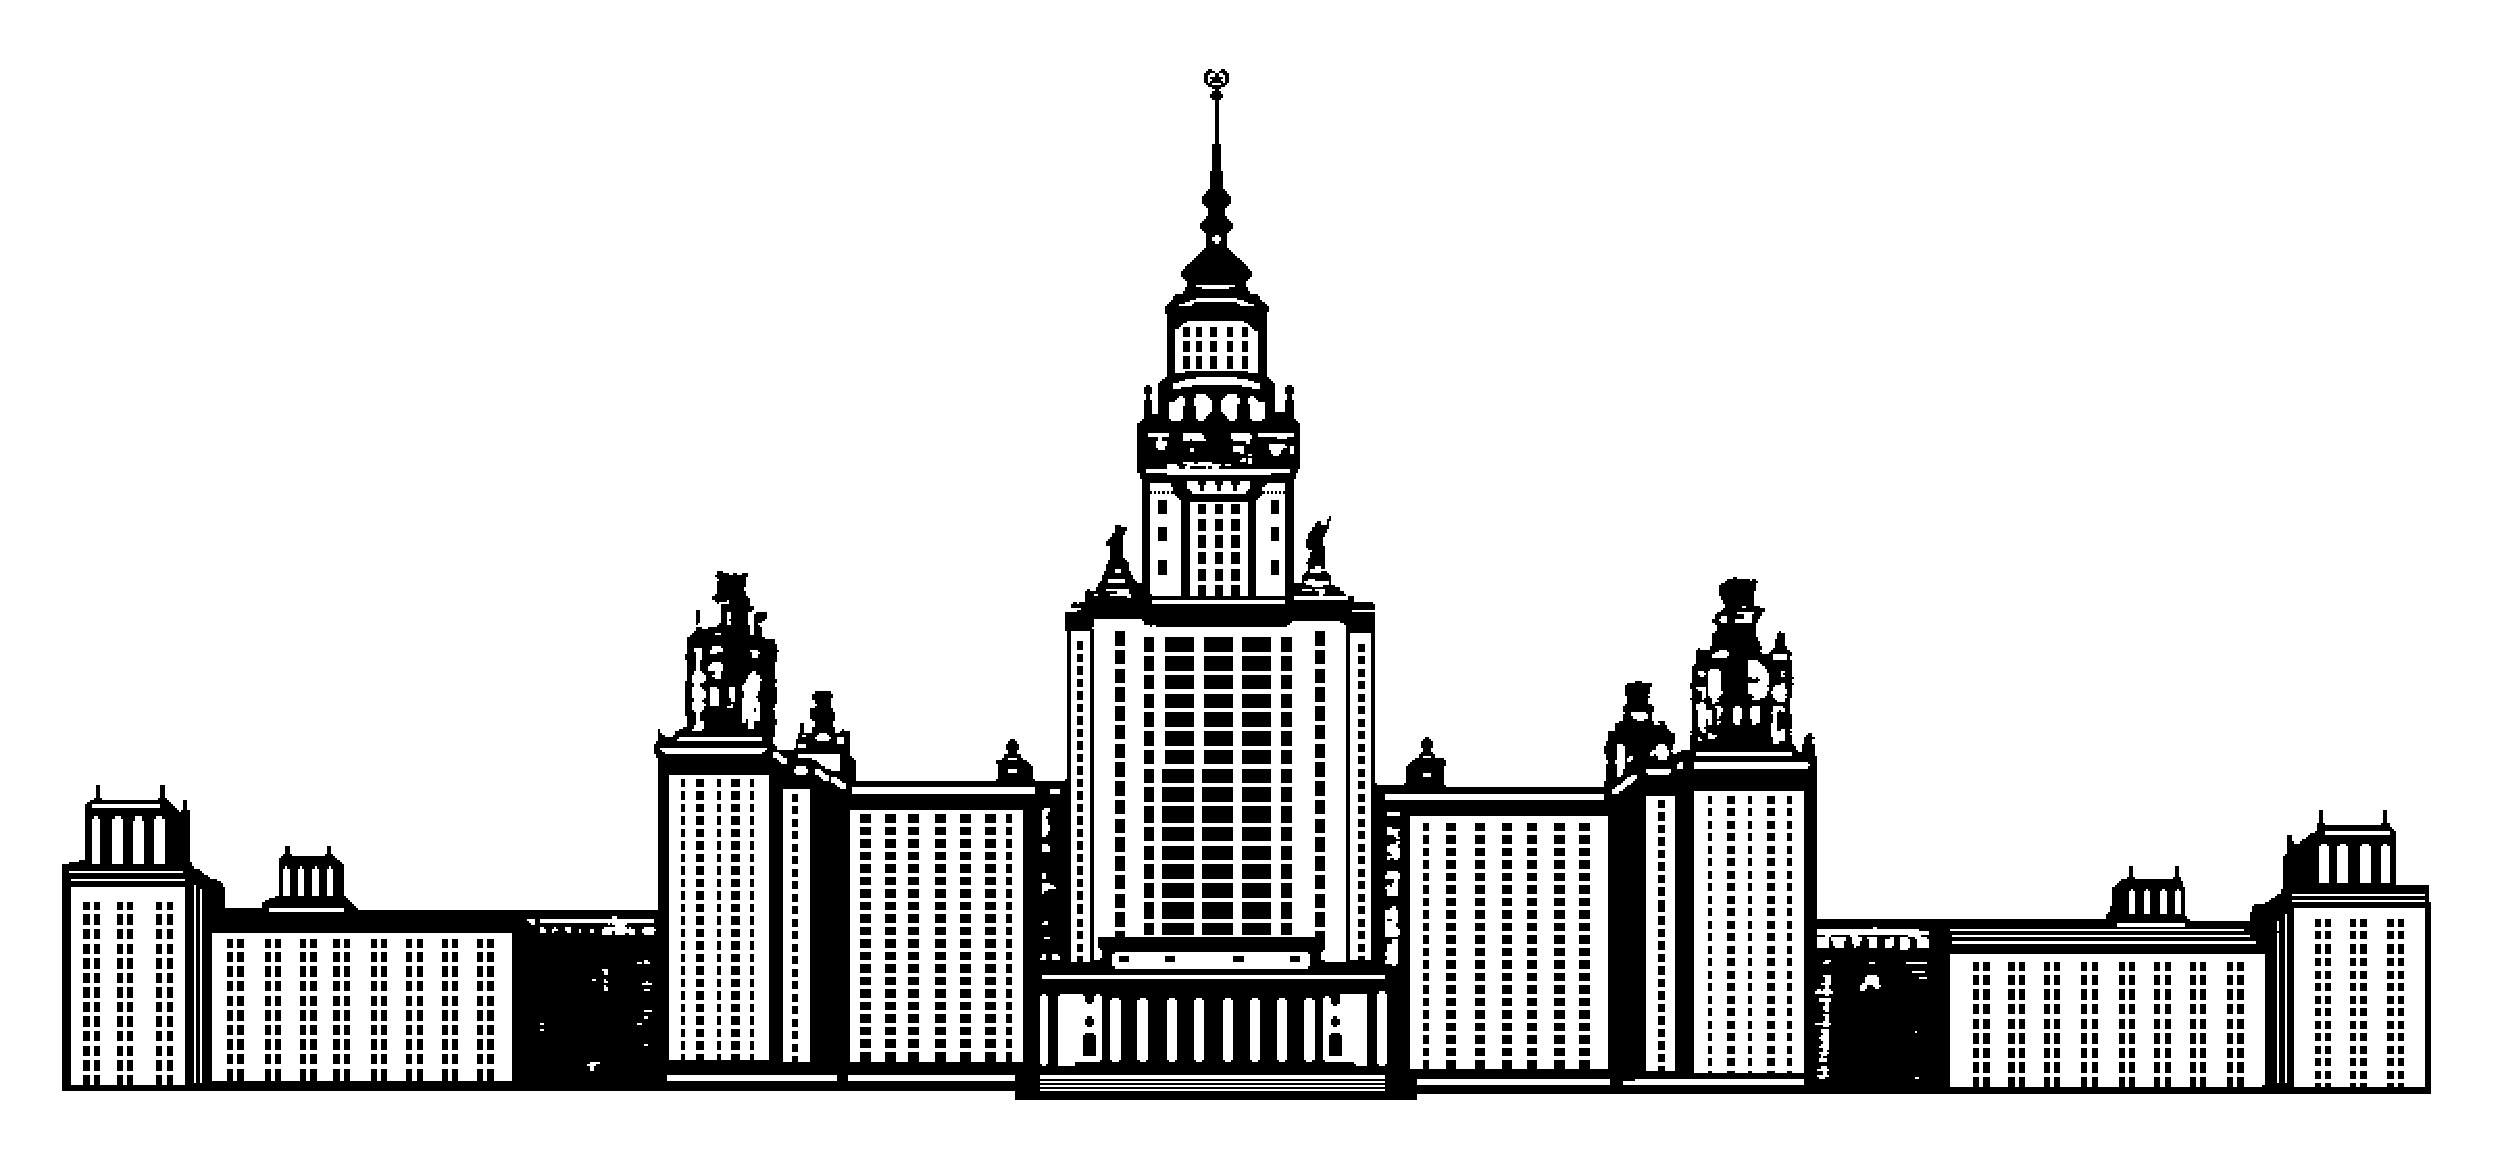
\includegraphics[width=50mm]{msu.eps}

    \bigskip
    Факультет Вычислительной Математики и Кибернетики\\
    Кафедра Математических Методов Прогнозирования\\[10mm]
    
    \textsf{\large\bfseries
        Отчет по первому заданию курса "Практикум на ЭВМ"\\[10mm]
        "Метрические алгоритмы классификации"
    }\\[10mm]
    \begin{flushright}
        \parbox{0.5\textwidth}{
        	Выполнила:\\
        	студентка 3 курса 317 группы \\
        	\emph{Кривуля Полина Юрьевна}\\[5mm]
        }
    \end{flushright}
    \vspace{\fill}
    Москва, 2022
\end{center}
\end{titlepage}

\newpage
\tableofcontents
\newpage

\section{Введение}

Метод k-ближайших соседей (k Nearest Neighbors, или kNN) – популярный алгоритм классификации и регрессии, который используется в различных типах задач машинного обучения. 

В случае использования метода для классификации объект присваивается тому классу, который является наиболее распространённым среди k соседей данного элемента, классы которых уже известны \cite{ss0}.

При взвешенном способе во внимание принимается не только количество попавших в область определённых классов, но и их удалённость от нового значения.

В наиболее общем виде алгоритм ближайших соседей есть 
$$a(u) = arg\max_{y\in Y} \sum_{i=1}^k[x_{i;j}=y]w(i;u),$$
где $w(i;u)$ - заданная весовая функция \cite{ss00}.

В рамках данного исследования выполнена собственная реализация класса $KNNClassifier$, имеющего метод поиска k ближайших соседей и расстояния между объектом и его соседями, и метод predict, предсказывающий, к какому классу должен принадлежать данный объект. В классе реализован поиск соседей как с весами, так и без. 

Также реализован модуль $cross\_validation$ с реализациями функций для применения кросс-валидации и модуль $distances$ с реализацией функций для вычисления евклидова и косинусного расстояния. 

В данном отчете проводятся эксперименты, позволяющие выяснить скорость и точность работы алгоритма на датасете MNIST в зависимости от различных параметров, а также исследуются возможные способы увеличения доли правильно предсказанных ответов. 



\section{Скорость работы алгоритмов в зависимости от числа признаков}

\subsection{Постановка задачи}

Измерьте для каждого алгоритма (kd\_tree, ball\_tree, brute и my\_own) поиска время нахождения 5 ближайших соседей для каждого объекта тестовой выборки по евклидовой метрике. Выберите подмножество признаков, по которому будет считаться расстояние, размера 10, 20, 100 (подмножество признаков выбирается один раз для всех объектов, случайно). Проверьте все алгоритмы поиска ближайших соседей, указанные в спецификации к заданию.

\subsection{Эксперименты и результаты}
С результатами данного эксперимента можно ознакомиться в таблице \ref{tab:widgets1}.
\begin{table}[h]
\begin{center}
\begin{tabular}{|*{5}{c|}}\hline
\backslashbox{Число признаков}{Метод} & kd\_tree & ball\_tree & brute & my\_own \\\hline
10 &  0.85 с &  4.89 с & 14.73 с & 15.87 с \\\hline
20 &  4.76 с & 13.76 с & 8.96 с & 11.01 с \\\hline
100 &  113.04 с & 94.59 с & 11.65 с & 15.92 с \\\hline
\end{tabular}
\caption{\label{tab:widgets1} Время поиска 5 ближайших соседей в зависимости от метода и числа признаков.}
\end{center}
\end{table}

Возникают следующие предположения:
\begin{enumerate}
    \item Методы kd\_tree и ball\_tree работают неэффективно по сравнению с другими методами при количестве признаков, большем 20
    \item Время работы методов brute и my\_own не зависит от числа признаков.
\end{enumerate}


Чтобы проверить данные предположения, измерим время нахождения 5 ближайших соседей для каждого объекта тестовой выборки по евклидовой метрике для подмножеств признаков размера 4, 6, 8, ..., 60. Подмножество признаков также выбирается один раз для всех объектов, случайно.
Получены следующие результаты:
\begin{center}
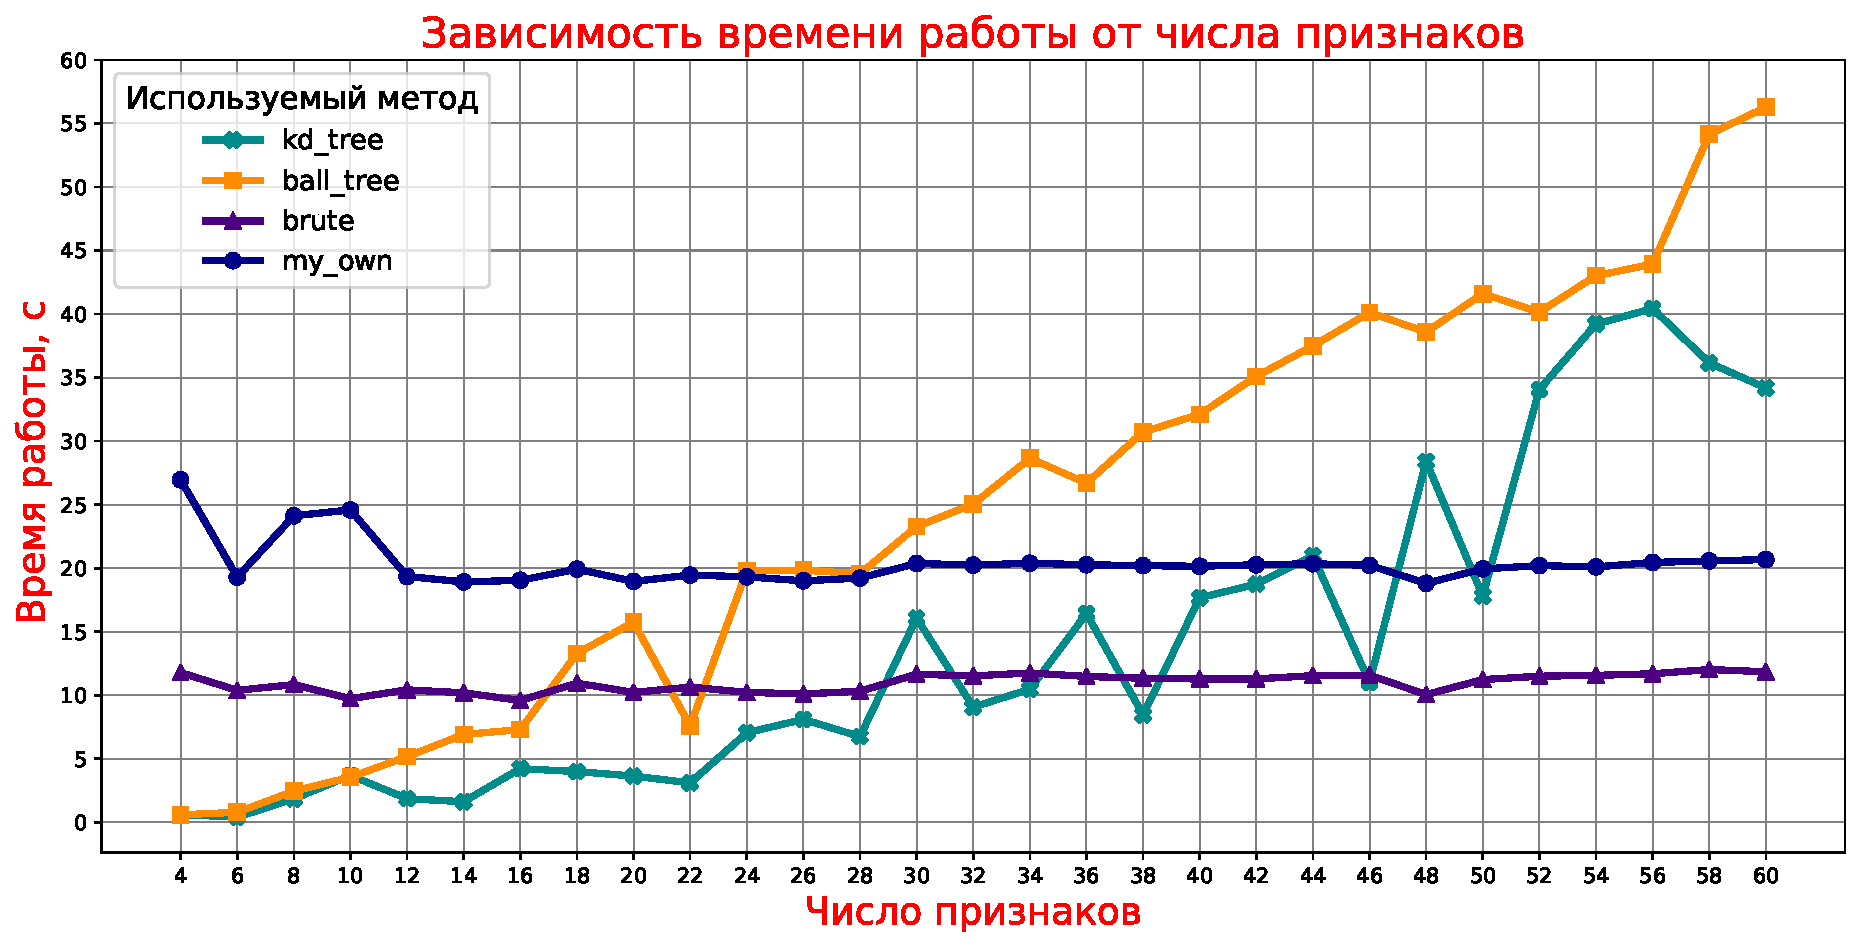
\includegraphics[width=15cm]{TASK1 PRAC FIGURE 0 time work.pdf}
\end{center}

Методы kd\_tree и ball\_tree работают быстрее методов brute и my\_own, но только при размерности признакового пространства на порядок меньшем, чем представлено в датасете MNIST (в нем размерность равна 784). Поэтому использование данных алгоритмов в рамках дальнейшего решения задачи неэффективно. 

Время работы методов brute и my\_own, в целом, не зависит от числа признаков. На графике видны небольшие выбросы, которые можно связать со временем работы самой среды или "неудачным"{ }выбором признаков, что подтверждается многократными запусками эксперимента. Алгоритмы устроены так, что время и работы практически не зависит от числа признаков, в большей степени оказывает влияние число соседей и количество объектов в выборке. Данный эксперимент подтвердил выдвинутые ранее предположения.

\subsection{Выводы}

\par Методы kd\_tree и ball\_tree работают эффективно при небольшом количестве признаков (<20). При большом количестве признаков методы работают в разы дольше, чем brute и my\_own. Связано это с тем, что kd\_tree и ball\_tree хранят объекты в виде деревьев. При большой размерности пространства алгоритму приходится посещать больше ветвей дерева, чтобы найти ближайших соседей, и с ростом числа признаков сложность становится примерно такой же, как и в случае полного перебора \cite{ss1}. Время работы методов brute и my\_own не зависит от числа признаков.

Полученные данные согласуются с информацией, найденной в открытых источниках \cite{ss2}.

\section{Кросс-валидация с 3 фолдами: точность и время работы}

\subsection{Постановка задачи}

Оцените по кросс-валидации с 3 фолдами точность (долю правильно предсказанных ответов) и время работы k ближайших соседей в зависимости от следующих факторов:

\begin{itemize}
    \item k от 1 до 10 (только влияние на точность).
    \item Используется евклидова или косинусная метрика.
\end{itemize}

Сравните взвешенный метод k ближайших соседей, где голос объекта равен $\frac{1}{distance  +  \epsilon}$, где $ \epsilon = {10}^{-5} $, с методом без весов при тех же фолдах и параметрах.

\subsection{Эксперименты и результаты} \hypertarget{3.2}{}
Здесь и далее используем самый быстро работающий метод: \textbf{brute.}
Запустим реализованную в рамках задания функцию $ knn\_cross\_val\_score $ со списком значений числа соседей 
$ k = [1, 2, ..., 10]. $ 

Для используемых метрик без весов получены значения времени работы, представленные в таблице \ref{tab:widgets2}.

\begin{table}[h]
\centering
\begin{tabular}{|c|c|c|}\hline
Используемая метрика & Евклидова & Косинусная \\\hline
Время работы, с & 135.9 & 122.6 \\\hline
\end{tabular}
\caption{\label{tab:widgets2} Время работы метода без весов.}
\end{table}

Здесь и далее долю правильно предсказанных ответов будем называть точностью. 

Получены значения точности, представленные на диаграмме ниже. 
\begin{center}
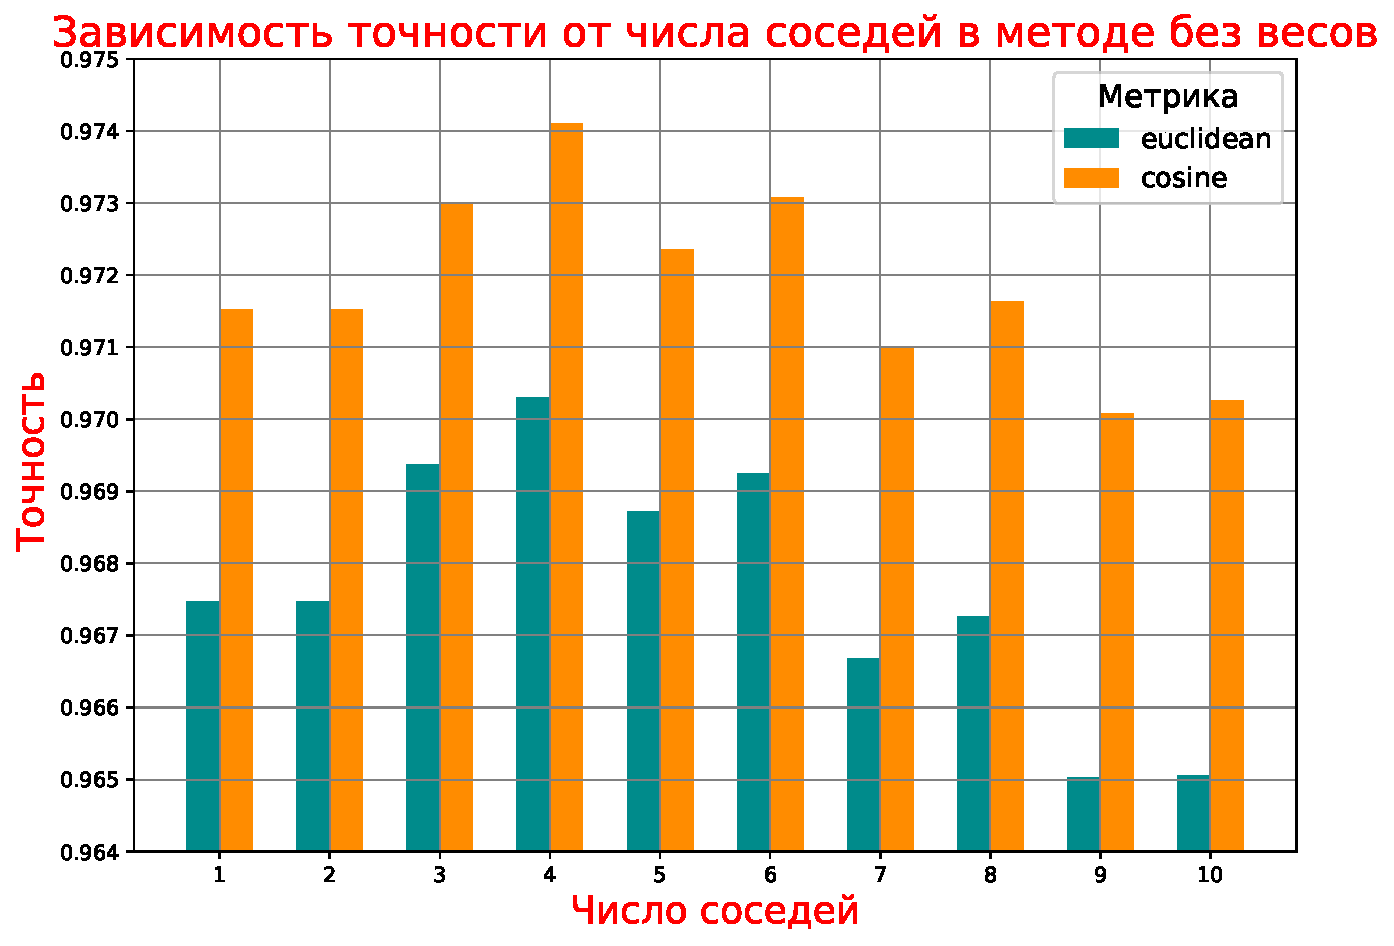
\includegraphics[width=10cm]{TASK1 PRAC FIGURE 1.pdf}
\end{center}

Косинусная метрика показала точность лучше, чем евклидова. Это можно объяснить тем, что косинусная метрика определяет степень сходства между объектами, и потому она менее чувствительна к сдвигам и растяжениям. Также она сработала незначительно (на 10\%) быстрее. 

Заметим, что при $k=2$ точность такая же, как и при $k=1$. Это происходит из-за особенностей реализации функции $ knn\_cross\_val\_score $: из-за линейности алгоритма ответы при каждом $k$ неявно зависят от ответов на предыдущих значениях, а в случае ситуации неоднозначного выбора класса для объекта, выбирается не случайный класс, а первый добавленный. То есть для $k=2$ получается, что класс всегда будет выбран как для $k=1$. Неслучайностью выбора в случае неоднозначного класса можно объяснить и то, что при нечетных k результат хуже, чем на предыдущих четных (кроме $k=3$, что уже объяснено). При $k>4$ точность начинает падать. Это объясняется тем, что в данной выборке объектов классов всего 10, поэтому при значениях $k$, близких к 10, алгоритм чрезмерно устойчив к шумовым выбросам и вырождается в константу \cite{ss00}.

Для используемых метрик с весами с голосом объекта $\frac{1}{distance + \epsilon}$, где $\epsilon={10}^{-5}$, получены значения времени работы, представленные в таблице \ref{tab:widgets3}.

\begin{table}[h]
\centering
\begin{tabular}{|c|c|c|}\hline
Используемая метрика & Евклидова & Косинусная \\\hline
Время работы, с & 129.9 & 123.1 \\\hline
\end{tabular}
\caption{\label{tab:widgets3} Время работы метода с весами.}
\end{table}

Время работы незначительно уменьшилось, так как при взвешенном методе возникает меньше неоднозначных ситуаций.

Получены значения точности, представленные на диаграммах ниже.
\begin{center}
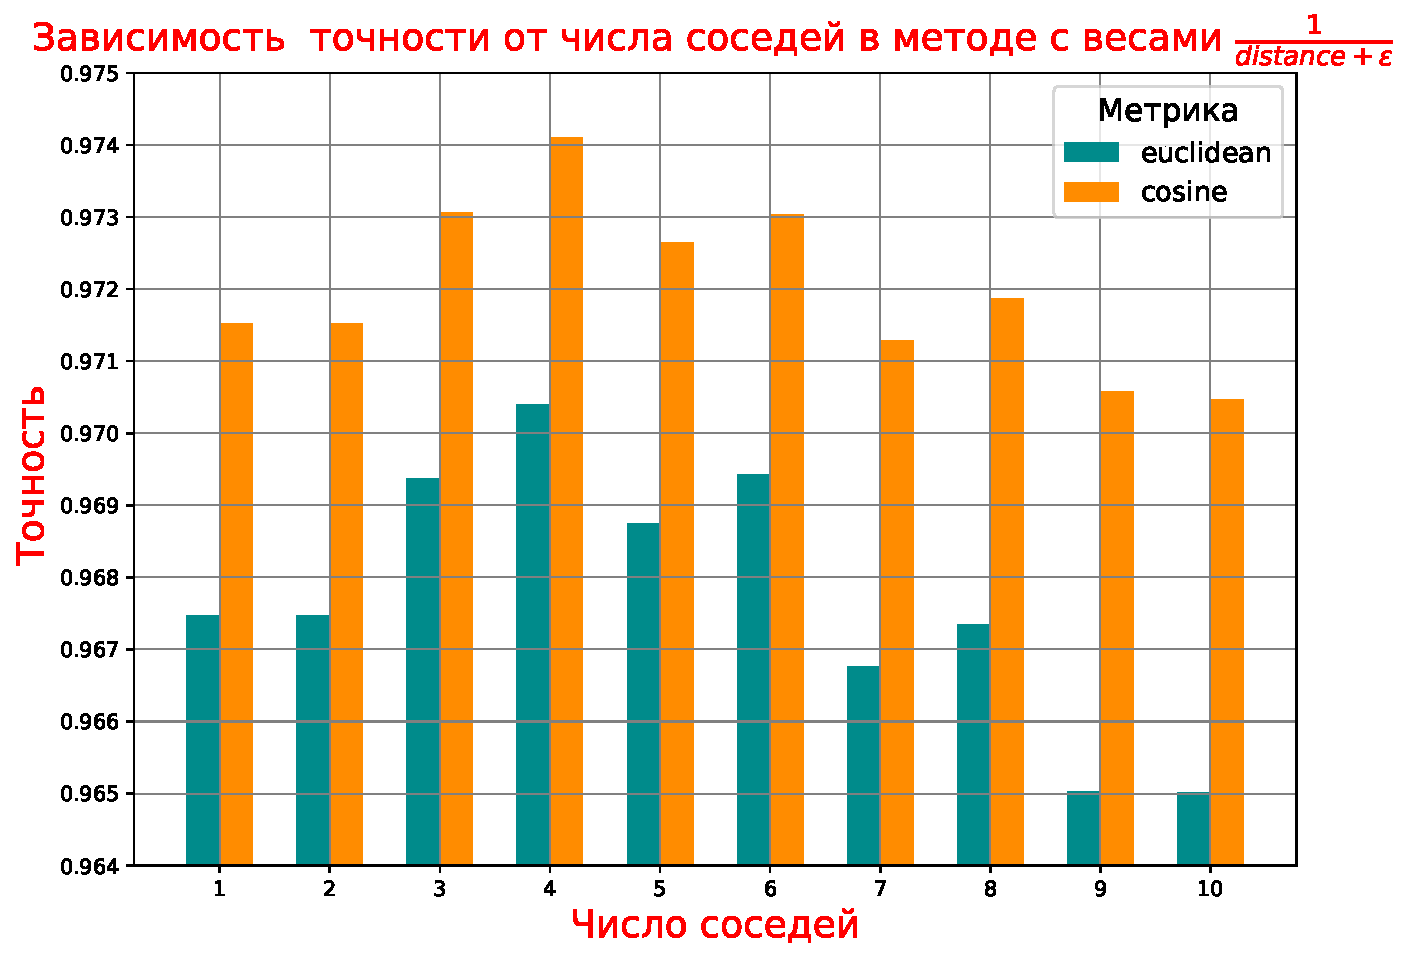
\includegraphics[width=10cm]{TASK1 PRAC FIGURE 2.pdf}
\end{center}

\begin{center}
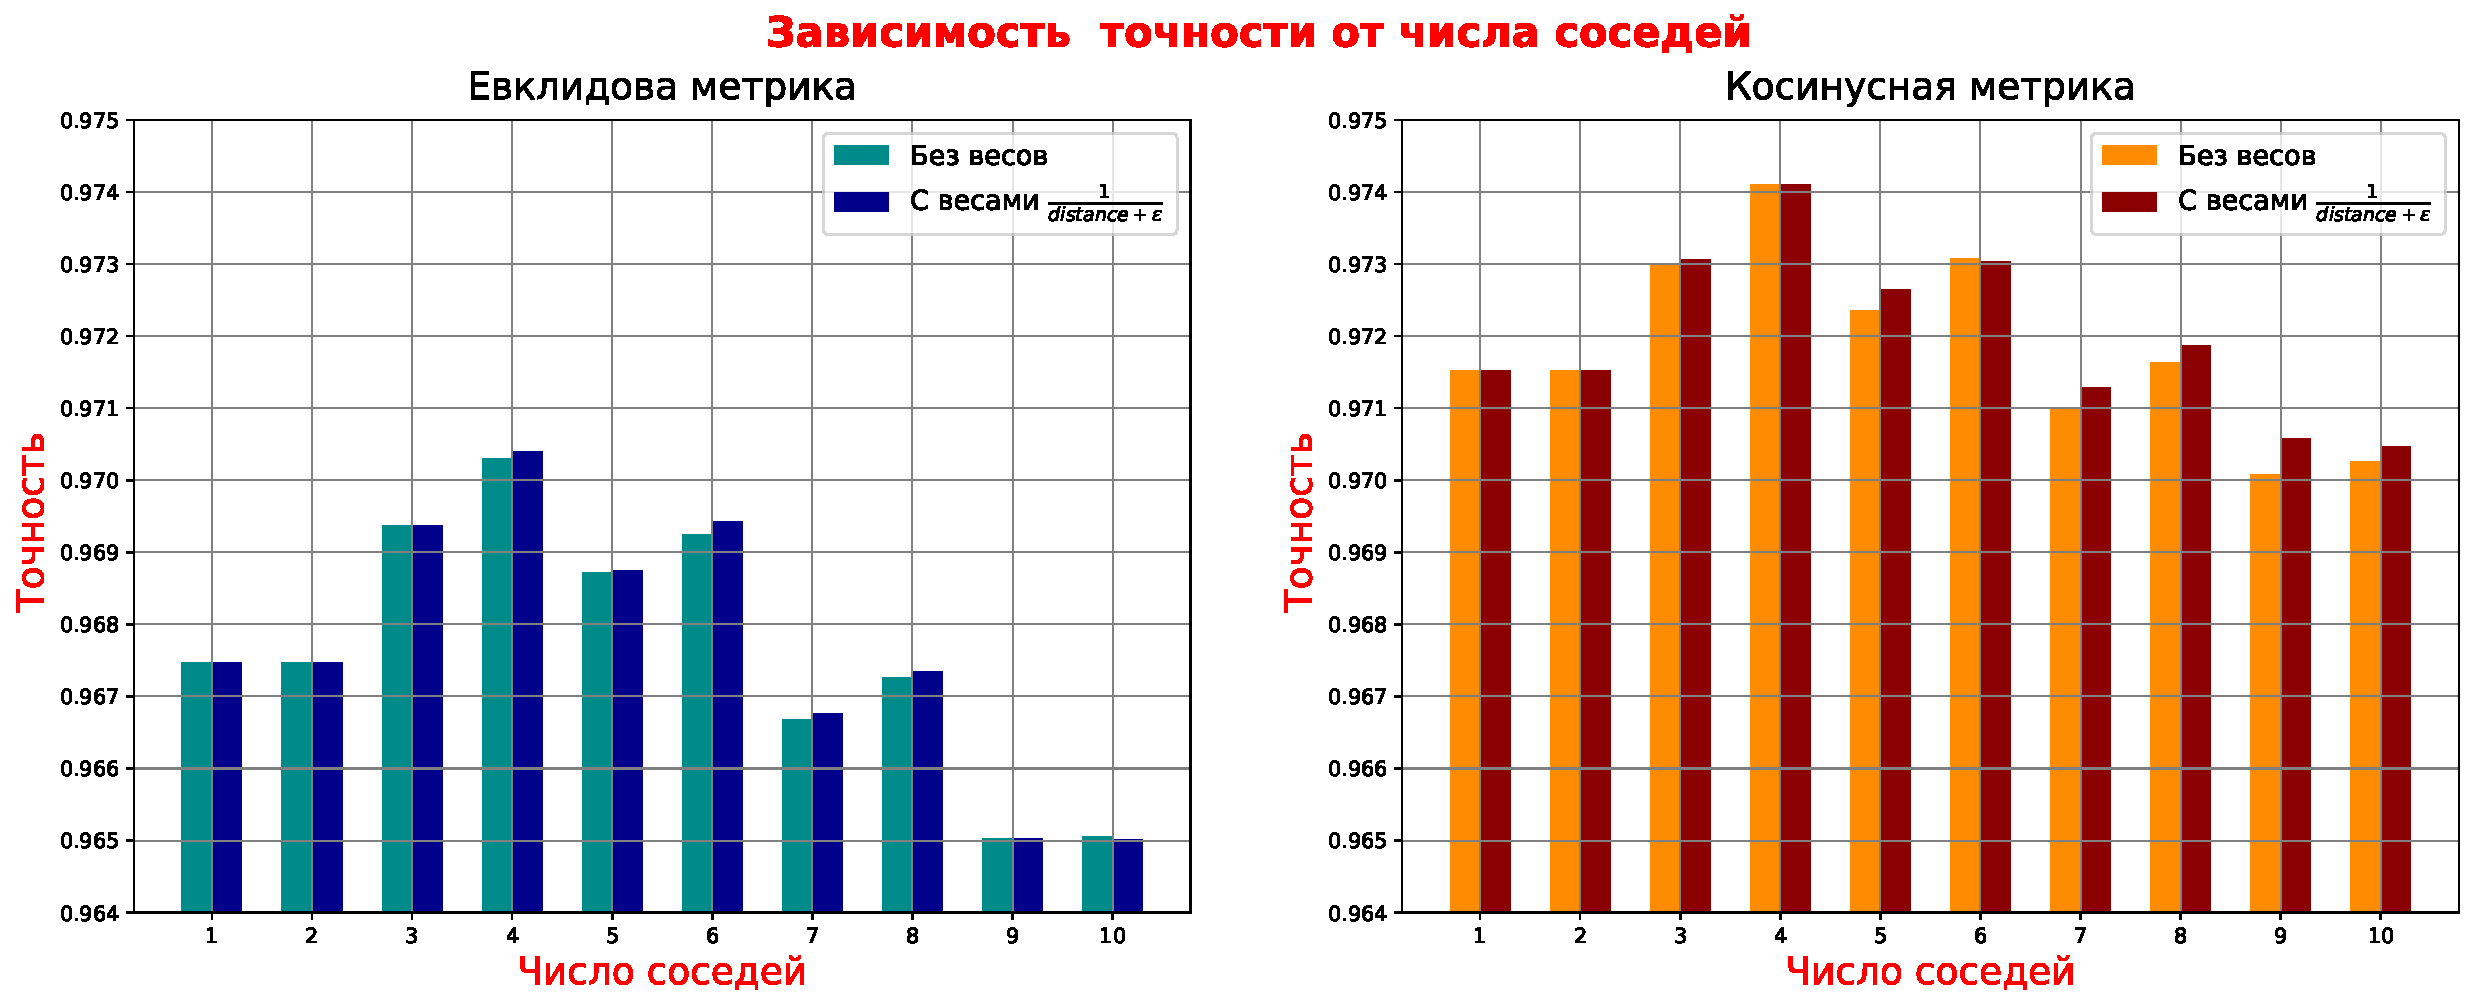
\includegraphics[width=15cm]{TASK1 PRAC FIGURE 2-1.pdf}
\end{center}

При $k=2$, как и в методе без весов, результат такой же, что и при $k=1$. Аналогично методу без весов, это связано с линейностью алгоритма (а также с особенностью используемой функции веса, описанной ниже). Ближайший сосед (с бóльшим весом) учтен при $k=1$, поэтому ответы при $k=2$ совпадают с предыдущими. 

Используемая функция веса объекта такова, что чем меньше расстояние, тем больше вес, следовательно, чем меньше номер соседа (номера упорядочены по удаленности от объекта, на котором ищется ответ), тем большее влияние он оказывает на ответ. Поэтому при $k=1$ ответ будет таким, какой он есть на первом соседе вне зависимости от факта взвешенности метода, и при $k=1,2$ результат одинаковый в методе без весов и с весами. Метод с весами позволяет избежать возникающих неоднозначных ситуаций, и в большинстве случаев точность повышается.

\subsection{Выводы}

При числе соседей $k=1,2$ ответы совпадают в обоих методах. Косинусная метрика показала результат лучше, чем евклидова, а максимальная точность достигается при $k=4$ косинусной метрики (одинаковая в методе с весами и без). При значениях $k$, близких к 10, точность падает, так как алгоритм становится чрезмерно устойчив к шумовым выбросам и вырождается в константу \cite{ss00}.



\section{Применение лучшего алгоритма к исходной обучающей и тестовой выборке}

\subsection{Постановка задачи}
Примените лучший алгоритм к исходной обучающей и тестовой выборке. Подсчитайте точность. Сравните с точностью по кросс-валидации. Сравните с указанной в интернете точностью лучших алгоритмов на данной выборке. Выполните анализ ошибок. Для этого необходимо построить и проанализировать матрицу ошибок (confusion matrix). Также визуализируйте несколько объектов из тестовой выборки, на которых были допущены ошибки. Проанализируйте и указажите их общие черты.

\subsection{Эксперименты и результаты}
По результатам предыдущего эксперимента лучшим алгоритмом вышла косинусная метрика для $k=4$ с весами и без. Так как метод с весами показал себя не хуже, чем метод без весов, используем далее его. Ранее было выяснено, что быстрее остальных методов работает brute. Поэтому в этом и следующих экспериментах используем косинусную метрику, число соседей $k=4$, взвешенный метод brute. Функция весов остается прежней.

При использовании данного алгоритма получена точность (доля правильно правильно предсказанных ответов) на тестовой выборке 0.9752. При этом лучшая (средння по фолдам) точность, полученная по кросс-валидации с 3 фолдами, равна 0.9741. Ее более низкое значение обусловлено тем, что по кросс-валидации обучение происходит на меньшем числе объектов: на 40 тыс., а тестирование на 20 тыс., в то время как размер всей обучающей выборки равен 60 тыс. объектов, а тестовой - 10 тыс.. Лучшая точность на данной выборке, представленная на Kaggle, равна 0.9998 \cite{ss2}.

Визуализация матрицы ошибок в данном эксперименте представлена ниже.
\begin{center}
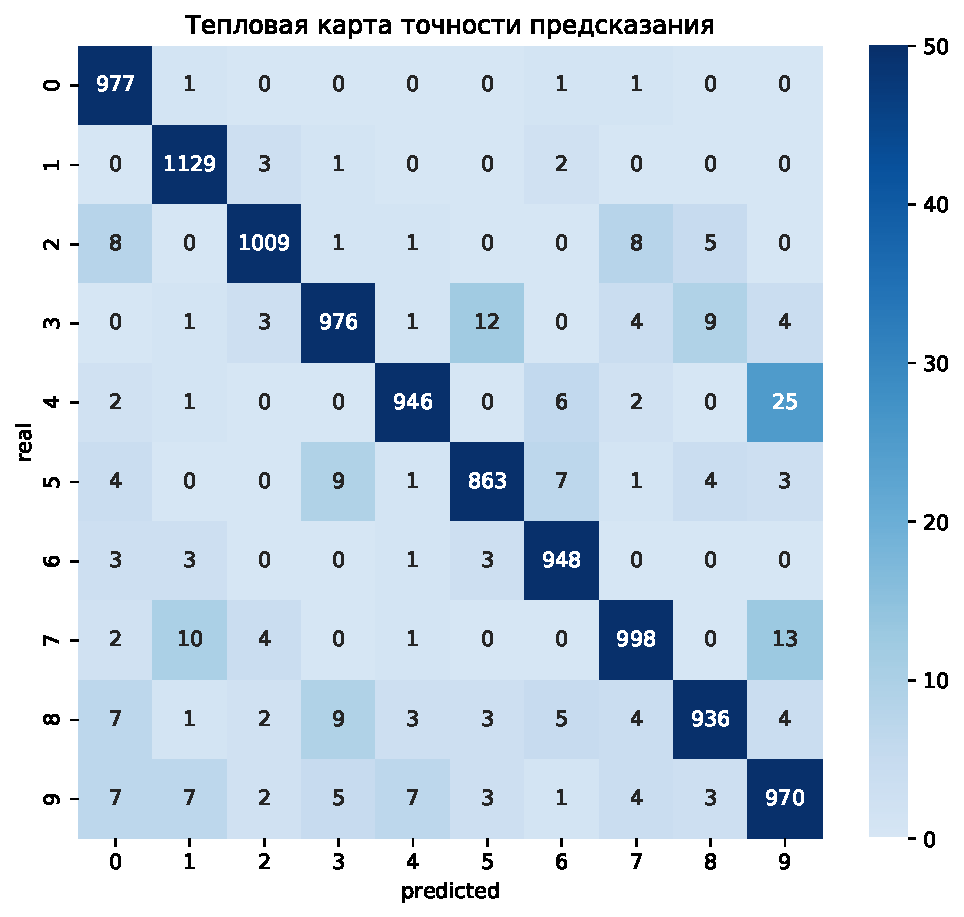
\includegraphics[width=7cm]{TASK1 warm map.pdf}
\end{center}

Чаще всего неправильно распознавалась "9": в 25 случаях реальная "4"{ }была распознана алгоритмом как "9"{}, и в 39 случаях реальная "9"{ }распознана неправильно. Ниже представлены оба случая, причем справа над каждом объектом написано, какая именно цифра была предсказана.


\begin{tabular}{cc}
    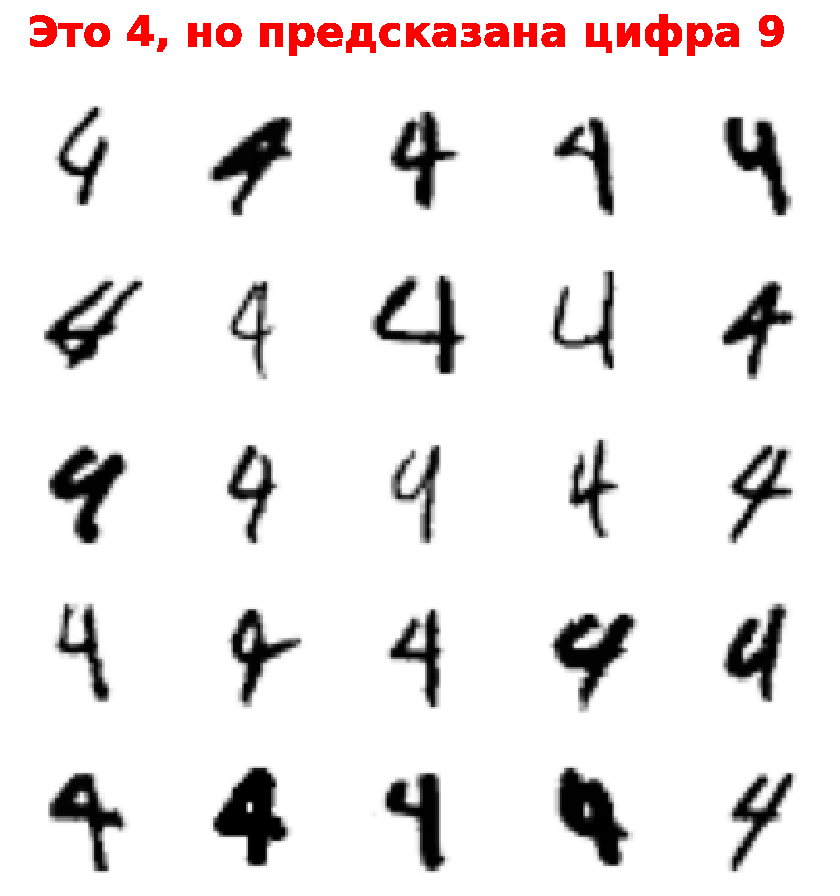
\includegraphics[width=7.2cm]{TASK1 PRAC FIGURE 4-1.pdf}
    & 
    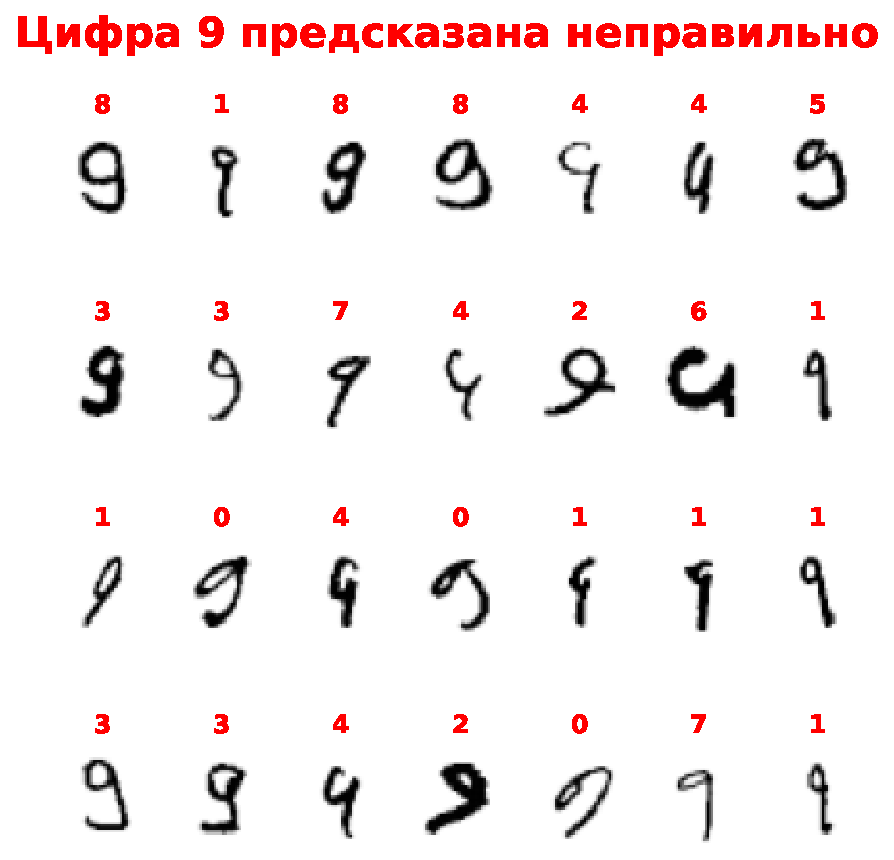
\includegraphics[width=8cm]{TASK1 PRAC FIGURE 4-2.pdf}\\
\end{tabular}

Заметим, что в первом случае большинство неправильно предсказанных "4"{ }написаны с{ }"замыканием"{ }сверху (как печатная, а не письменная версия цифры), и поэтому они становятся похожими на "9".
Во втором случае часть "9"{ }написаны так, что и человек может неправильно их распознать. Если такие объекты попадают в обучающую выборку, то это оказывает негативное влияние на дальнейшее распознавание алгоритмом правильно написанных цифр. 

Ниже представлены 50 случайно выбранных из неправильно распознанных цифр. Многие из этих цифр написаны непонятно, поэтому сверху каждой написано, какая это на самом деле цифра ("Real") и как эту цифру распознал алгоритм ("Pred"). 

\begin{center}
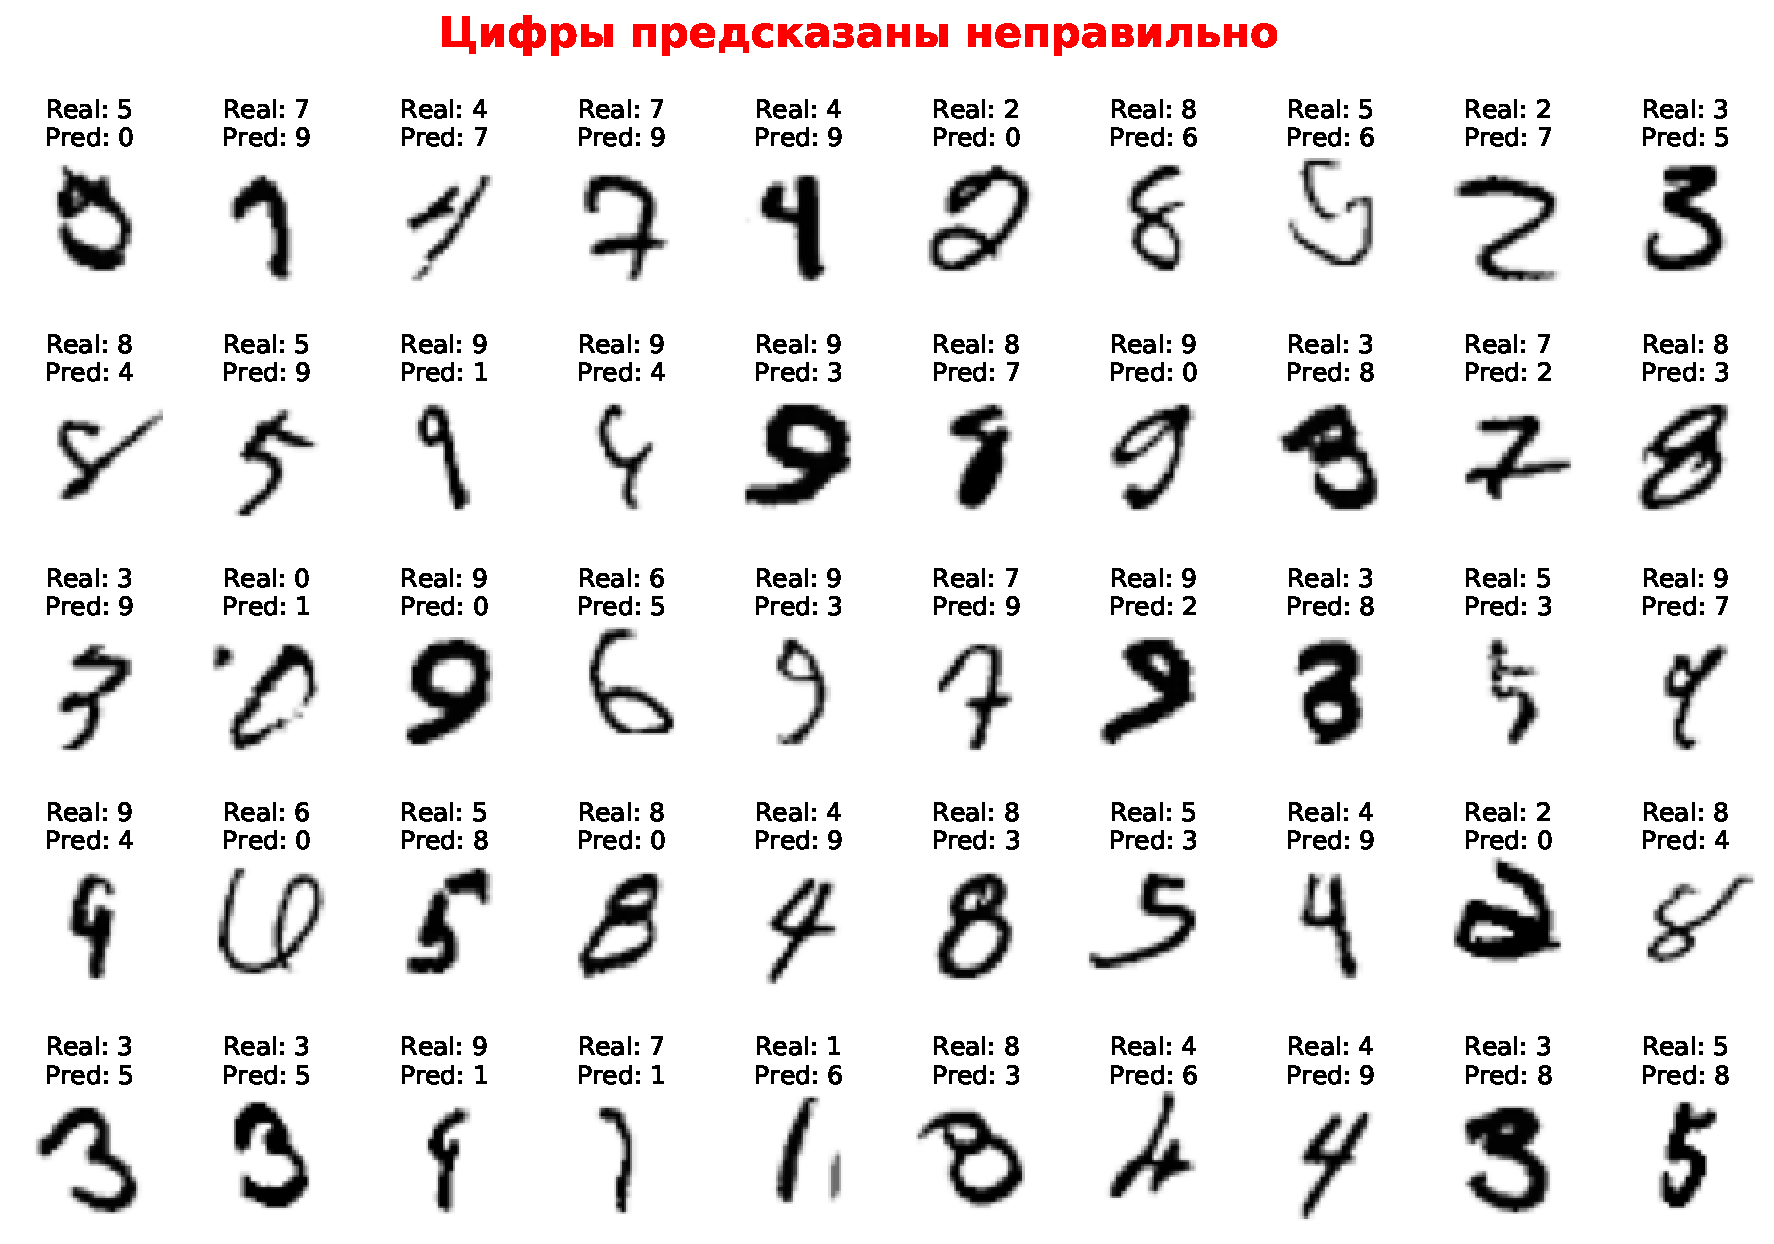
\includegraphics[width=12cm]{TASK1 PRAC FIGURE 4-3.pdf}
\end{center}

Помимо непонятно написанных цифр (которые являются неинформативными объектами и/или выбросами), алгоритм часто неправильно распознает нечеткие и повернутые цифры. Данную проблему можно решать, в частности, с помощью аугментации.

\subsection{Выводы}
Доля правильно предсказанных данным алгоритмом ответов на тестовой выборке на 0.0246 меньше, чем лучшая на Kaggle. Алгоритм неправильно распознает в целом для человека непонятно написанные цифры (возможно, выбросы), а также нечеткие, повернутые и сдвинутые.


\section{Аугментация обучающей выборки}

\subsection{Постановка задачи}
Выполните аугментацию обучающей выборки. Для этого нужно размножить ее с помощью поворотов, смещений, морфологических операций и применений гауссовского фильтра. Разрешается использовать библиотеки для работы с изображениями. Подберите по кросс-валидации с 3 фолдами параметры преобразований. Рассмотрите следующие параметры для преобразований и их комбинации:
\begin{itemize}
    \item Величина поворота: 5, 10, 15 (в каждую из двух сторон);
    \item Величина смещения: 1, 2, 3 пикселя (по каждой из двух размерностей);
    \item Дисперсия фильтра Гаусса: 0.5, 1, 1.5;
    \item Морфологические операции: эрозия, дилатация, открытие, закрытие с ядром 2.
\end{itemize}

\subsection{Эксперименты и результаты}

В данном эксперименте возникла необходимость немного изменить функцию $ knn\_cross\_val\_score $ и сделать в ней случайный выбор индексов (иначе при некоторых параметрах преобразования точность выдавалась как равная 1).

Напомним, что исходная точность по кросс-валидации с 3 фолдами была равна 0.9741.

\begin{itemize}
    \item Величина поворота: 5, 10, 15 (в каждую из двух сторон)
    
    При реализации данной аугментации размер обучающей выборки увеличивается в 3 раза: помимо самой выборки к ней добавляется она же, повернутая на $\phi ^\circ$ в одну сторону и на $\phi ^\circ$ в другую.
    
    В результате по кросс-валидации с 3 фолдами получены результаты, представленные в таблице \ref{tab:widgets4}.
    
    \begin{table}[h]
    \begin{center}
    \begin{tabular}{|*{4}{c|}}\hline
    Величина поворота & $ 5 ^\circ$  & $10 ^\circ$ & $15 ^\circ$ \\\hline
    Точность &  0.9935 &  0.9910 & 0.9879 \\\hline
    \end{tabular}
    \caption{\label{tab:widgets4} Точность в зависимости от величины поворота.}
    \end{center}
    \end{table}
    
    Визуализации матриц ошибок для каждого случая представлены в приложении ($ 5 ^\circ$ - \ref{app:rot5}, $10 ^\circ$ - \ref{app:rot10}, $15 ^\circ$ - \ref{app:rot15}).
    
    При повороте на $ 5 ^\circ$ неправильно предсказанных ответов стало количественно меньше, особенно в случае с цифрой "9". При повороте на $10 ^\circ$ и $15 ^\circ$, наоборот, ошибок в этом случае становится больше (особенно когда реальная цифра "4"{ } распознается как "9") и добавляются другие ошибки. Но данные преобразования помогают исправить обозначенную ранее ошибку распознавания повернутого объекта.

    \item Величина смещения: 1, 2, 3 пикселя (по каждой из двух размерностей)
    
    При реализации данной аугментации размер обучающей выборки увеличивается в 3 раза: помимо самой выборки к ней добавляется она же, смещенная на $\alpha$ пикселей в одну сторону и на $\alpha$ в другую. Сторона смещения подбиралась как дающая лучшую точность на значении $\alpha=1$, что представлено в таблице \ref{tab:widgets5}.
       
    \begin{table}[H]
    \begin{center}
    \begin{tabular}{|*{2}{c|}}\hline
    Пара векторов смещений & Полученная точность \\\hline
    [1, 1],  [-1, -1] &  0.9776 \\\hline
    [1, 0],  [-1,  0] &  0.9842 \\\hline
    [1, 0],  [ 0, -1] &  0.9842 \\\hline
    [0, 1],  [ 0, -1] &  0.9840 \\\hline
    [1, 0],  [ 0,  1] &  0.9850 \\\hline
    \end{tabular}
    \caption{\label{tab:widgets5} Точность в зависимости направлений смещения на 1 пиксель.}
    \end{center}
    \end{table}
    Лучшая точность была достигнута на последней паре векторов. Поэтому данная пара и будет использоваться в смещениях на 2 и 3 пикселя. Полученные значения представлены в таблице \ref{tab:widgets6}.
    
    \begin{table}[H]
    \begin{center}
    \begin{tabular}{|*{4}{c|}}\hline
    Величина смещения, пикселей & 1 & 2 & 3\\\hline
    Точность &  0.9850 &  0.9766 & 0.9758 \\\hline
    \end{tabular}
    \caption{\label{tab:widgets6} Точность в зависимости от величины сдвига.}
    \end{center}
    \end{table}

    Визуализации матриц ошибок для каждого случая величины сдвига (по паре векторов смещения [1, 0],  [ 0,  1]) представлены в приложении (смещение на 1 пиксель - \ref{app:shift1}, на 2 - \ref{app:shift2}, на 3 - \ref{app:shift3}).
    
    Данные преобразования помогают исправить обозначенную ранее ошибку распознавания сдвинутого объекта, причем лучшую точность дает смещение на 1 пиксель, а оставшиеся смещения количественно добавляют новые ошибки.

    
    \item Дисперсия фильтра Гаусса: 0.5, 1, 1.5
    
    При реализации данной аугментации размер обучающей выборки увеличивается в 2 раза: помимо самой выборки к ней добавляется она же, преобразованная с использованием фильтра Гаусса с заданной дисперсией.
    
    Дисперсия 1.5 сильно портит объекты, что представлено ниже. 
    
    
\includegraphics[width=2cm]{TASK1 badgaus.png}
    
    Для фильтра Гаусса с дисперсией 0.5 и 1 по кросс-валидации с 3 фолдами получены результаты, представленные в таблице \ref{tab:widgets7}.
    
    \begin{table}[H]
    \begin{center}
    \begin{tabular}{|*{3}{c|}}\hline
    Дисперсия фильтра Гаусса & 0.5 & 1 \\\hline
    Точность &  0.9926 &  0.9912  \\\hline
    \end{tabular}
    \caption{\label{tab:widgets7} Точность в зависимости от дисперсии фильтра Гаусса.}
    \end{center}
    \end{table}
    
    Оба фильтра дают хорошие значения точности. Визуализации матриц ошибок для каждого случая представлены в приложении (с дисперсией 0,5 - \ref{app:filter0_5}, с дисперсией 1 - \ref{app:filter1}).
    Данные преобразования помогают исправить обозначенную ранее ошибку распознавания размытого объекта.
    
    \item Морфологические операции: эрозия, дилатация, открытие, закрытие с ядром 2
    
    При реализации данной аугментации размер обучающей выборки увеличивается в 2 раза: помимо самой выборки к ней добавляется она же, преобразованная с использованием морфологической операции.
    
    \begin{table}[H]
    \begin{center}
    \begin{tabular}{|c|*{4}{@{ { }}c@{ { }}|}}\hline
    Морфологические операции & Эрозия & Дилатация  & Открытие & Закрытие \\\hline
    Точность &  0.9863 &  0.9876  &  0.9823  & 0.9819  \\\hline
    \end{tabular}
    \caption{\label{tab:widgets8} Точность в зависимости от используемой морфологической операции.}
    \end{center}
    \end{table}
    
    Визуализации матриц ошибок для каждого случая представлены в приложении (эрозия - \ref{app:erode}, дилатация - \ref{app:dilate}, открытие - \ref{app:open}, закрытие - \ref{app:close}). При сравнении полученных матриц ошибок с изначальной, можно заметить, что данные преобразования не дают заметного повышения точности. Скорее всего, на кросс-валидации точность повысилась больше за счет увеличения выборки, чем за счет данных преобразований.

    \item Комбинация различных преобразований
    
    Для комбинации различных преобразований реализована функция augm, которая в зависимости от параметров, поступающих на вход, преобразовывает выборку следующим образом: случайно выбирается поворот в диапазоне $[-5 ^\circ; 5^\circ]$, и/или случайным образом сдвигает на -1, 0, 1 пиксель по обеим размерностям, и/или случайным образом решает, преобразовывать ли с помощью фильтра Гаусса с дисперсией 0.5, и/или случайно выбирает морфологическую операцию. Все перечисленные действия применяются к каждому объекту.
    \begin{enumerate}
        \item[0.] Увеличим исходную выборку в 3 раза: преобразуем ее с помощью поворота на $5^\circ$ в обе стороны и фильтра Гаусса с дисперсией 0.5.
        
        Таким образом получена точность 0.9935, что не отличается от полученной при данном повороте без фильтра Гаусса (см. таблица \ref{tab:widgets4}). Матрица ошибок представлена в приложении (\ref{app:violet0})
        \item Случайный выбор параметров 1
        
        Увеличим исходную выборку в 3 раза. Одну копию исходной выборки преобразуем с помощью функции augm для случайного поворота и фильтра Гаусса, на второй с помощью функции augm сделаем все случайные преобразования. Получена точность 0.9828, что хуже предыдущего результата. Матрица ошибок представлена в приложении (\ref{app:violet1}).
        
        \item Случайный выбор параметров 2
        
        Увеличим исходную выборку в 3 раза. Одну копию исходной выборки преобразуем с помощью функции augm для случайного поворота и фильтра Гаусса, на второй с помощью функции augm сделаем оставшиеся случайные преобразования (сдвиг на 1 пиксель, морфологические операции). Получена точность 0.9827. Матрица ошибок представлена в приложении (\ref{app:violet2}).
        
        \item Случайный выбор параметров 3
        
        Увеличим исходную выборку в 3 раза. Одну копию исходной выборки преобразуем с помощью функции augm для случайного поворота и фильтра Гаусса, на второй с помощью функции augm сделаем случайный поворот. Получена точность 0.9880. Матрица ошибок представлена в приложении (\ref{app:violet3})
        
        \item Выбор параметров 4 \hypertarget{par_ch_4}{}
        
        Увеличим исходную выборку в 4 раза. Одну копию исходной выборки преобразуем с помощью функции augm для всех случайных параметров, вторую преобразуем с помощью (не случайного) поворота на $5^\circ$, третью с помощью поворота на $-5^\circ$. Также ко второй и третьей выборке применим фильтр Гаусса с дисперсией 0.5. Получена точность по кросс-валидации с 3 фолдами 0.9944, что лучше всего опробованного ранее. Матрица ошибок представлена в приложении (\ref{app:violet4}). Увеличились все правильные предсказания, кроме "6"{ }(числа на диагонали матрицы), то есть, увеличилось число правильно предсказанных ответов на тестовой выборке. В случае "6"{ }добавились 3 случая неправильного предсказания, что по отношению к правильно распознанной цифрой "6"{ }(945 случаев) незначительно.
        
        При использовании данной аугментированной обучающей выборки, доля правильно предсказанных ответов на тестовой выборке увеличивается с 0.9752 до 0.9809. 
        
        
   \end{enumerate}
    
\end{itemize}

\subsection{Выводы}
С помощью аугментации обучающей выборки в экспериментах получено увеличение точности по кросс-валидации. Исходная точность по кросс-валидации с 3 фолдами была равна 0.9741, а с помощью увеличения выборки в 4 раза и последующих преобразований было достигнуто значение 0.9944.

\section{Преобразование тестовой выборки}

\subsection{Постановка задачи}
Реализуйте описанный выше алгоритм, основанный на преобразовании объектов тестовой выборки. Проверьте то же самое множество параметров, что и в предыдущем пункте. Проанализируйте как изменилась матрица ошибок, какие ошибки алгоритма помогает исправить каждое преобразование. Качественно сравните два подхода (5 и 6 пункты) между собой.


\subsection{Эксперименты и результаты}
Напомним, что исходная точность, посчитанная как доля правильно предсказанных ответов на тестовой выборке, равна 0.9752.
\begin{itemize}
    \item Величина поворота: 5, 10, 15 (в каждую из двух сторон)
    
    Случайным образом выбирается, в какую именно сторону поворачивать объект.
    В таблице \ref{tab:widgets9} представлено, как преобразование тестовой выборки влияет на долю полученных правильных ответов (на преобразованной выборке).
    
    \begin{table}[h]
    \begin{center}
    \begin{tabular}{|*{4}{c|}}\hline
    Величина поворота & $ 5 ^\circ$  & $10 ^\circ$ & $15 ^\circ$ \\\hline
    Точность &  0.9723 &  0.9669 & 0.9421 \\\hline
    \end{tabular}
    \caption{\label{tab:widgets9} Точность в зависимости от величины поворота.}
    \end{center}
    \end{table}
    
    Визуализации матриц ошибок для каждого случая представлены в приложении ($ 5 ^\circ$ - \ref{app6:rot5}, $10 ^\circ$ - \ref{app6:rot10}, $15 ^\circ$ - \ref{app6:rot15}).
    
    Голосование среди полученных ответов на исходной выборке и на одном повороте бессмысленно, более подробно было описано в \hyperlink{3.2}{пункте 3.2}.
    
    При использовании всех трех преобразований и голосовании среди них и полученных ответов на исходной выборке, результат хуже, чем для просто поворота на $ 5 ^\circ$: получена точность 0.9661.
    Были проверены всевозможные комбинации преобразований и голосования среди полученных результатов и единственное улучшение было достигнуто при следующем варианте: 
    
    Принятие решения путем голосования среди ответов на тестовой выборке, повернутой на $ 5 ^\circ$, повернутой на $ -5 ^\circ$ и исходной. Таким образом была достигнута точность 0.9763. Матрица ошибок представлена в приложении (\ref{app6:rot5+-}).
    
    \item Величина смещения: 1, 2, 3 пикселя (по каждой из двух размерностей)
    
    Голосование среди полученных ответов на исходной выборке, на смещении на $\alpha$ пикселей по вектору [$\alpha$; 0], на смещении на $\alpha$ пикселей по вектору [0; $\alpha$]. Полученные результаты представлены в таблице \ref{tab:widgets10}
    
    
    \begin{table}[h]
    \begin{center}
    \begin{tabular}{|*{4}{c|}}\hline
    Величина смещения &  1  &  2  & 3 \\\hline
    Доля правильных ответов  & 0.9712  & 0.9455 & 0.8681 \\\hline
    \end{tabular}
    \caption{\label{tab:widgets10} Точность в зависимости от величины смещения.}
    \end{center}
    \end{table}
    
    Визуализации матриц ошибок для каждого случая представлены в приложении (1 - \ref{app6:shift1}, 2 - \ref{app6:shift2}, 3 - \ref{app6:shift3}).
    
    Были проверены всевозможные комбинации преобразований и голосования среди полученных результатов и улучшение было достигнуто при следующем варианте: 
    
    Голосование среди полученных ответов на исходной выборке и всевозможных смещениях на 1. Получена точность 0.9761. Матрица ошибок представлена в приложении (\ref{app6:goodshift}).

    \item Дисперсия фильтра Гаусса: 0.5, 1, 1.5
    
    В таблице \ref{tab:widgets11} представлено, как данные преобразования тестовой выборки влияют на долю полученных правильных ответов (на преобразованной выборке). При этом известно, что фильтр Гаусса с дисперсией 1.5 уже достаточно сильно портит объекты.

    \begin{table}[H]
    \begin{center}
    \begin{tabular}{|*{4}{c|}}\hline
    Дисперсия фильтра Гаусса & 0.5 & 1 & 1.5 \\\hline
    Доля правильных ответов & 0.9742  &  0.9711 & 0.9623 \\\hline
    \end{tabular}
    \caption{\label{tab:widgets11} Точность в зависимости от дисперсии фильтра Гаусса.}
    \end{center}
    \end{table}
    
    Визуализации матриц ошибок для каждого случая представлены в приложении (дисперсия 0.5 - \ref{app6:gauss05}, дисперсия 1 - \ref{app6:gauss1}, дисперсия 1.5 - \ref{app6:gauss15}).
    
    Были реализованы различные комбинации преобразований из данного пункта и принятие решения путем голосования, но улучшение по сравнению с исходной точностью достигнуто не было. Например, голосованием среди преобразования с дисперсией 0.5, с дисперсией 1 и ответов на исходной тестовой выборке, была получена точность 0.9743 При этом просто на исходной достигается точность 0.9752.
    
    \item Морфологические операции: эрозия, дилатация, открытие, закрытие с ядром 2

    В таблице \ref{tab:widgets12} представлено, как данные преобразования тестовой выборки влияет на долю полученных правильных ответов (на преобразованной выборке).

    \begin{table}[H]
    \begin{center}
    \begin{tabular}{|c|*{4}{@{ { }}c@{ { }}|}}\hline
    Морфологические операции & Эрозия & Дилатация  & Открытие & Закрытие \\\hline
    Доля правильных ответов  & 0.9665  & 0.9638  &  0.9475  &  0.9481 \\\hline
    \end{tabular}
    \caption{\label{tab:widgets12} Точность в зависимости от морфологической операции}
    \end{center}
    \end{table}
    
    Визуализации матриц ошибок для каждого случая представлены в приложении (эрозия - \ref{app6:morf1}, дилатация - \ref{app6:morf2}, открытие - \ref{app6:morf3}, закрытие - \ref{app6:morf4}).
    
    Данные преобразования дают точность хуже, чем все предыдущие и по матрицам ошибок видно, что ошибки появляются практически в одних и тех же местах, поэтому голосование среди них бесполезно.

    \item Обобщение
    
    Если сделать голосование среди лучших полученных результатов (в экспериментах 1 и 2 данного пункта), то точность будет как в эксперименте 1 (0.9763).
    
    \item Обобщение с аугментацией

    Совместим аугментацию, на которой был достигнут лучший результат (\hyperlink{par_ch_4}{комбинация преобразований 4}) и обобщение из предыдущего подпункта. Таким способом получена точность 0.9823. Напомним, что исходная точность на тестовой выборке (не по кросс-валидации) была равна 0.9752, а доля правильно предсказанных ответов на аугментированной обучающей выборке - 0.9809. 
    Более наглядно это отображено на диаграмме ниже.
    
    
    \begin{center}
        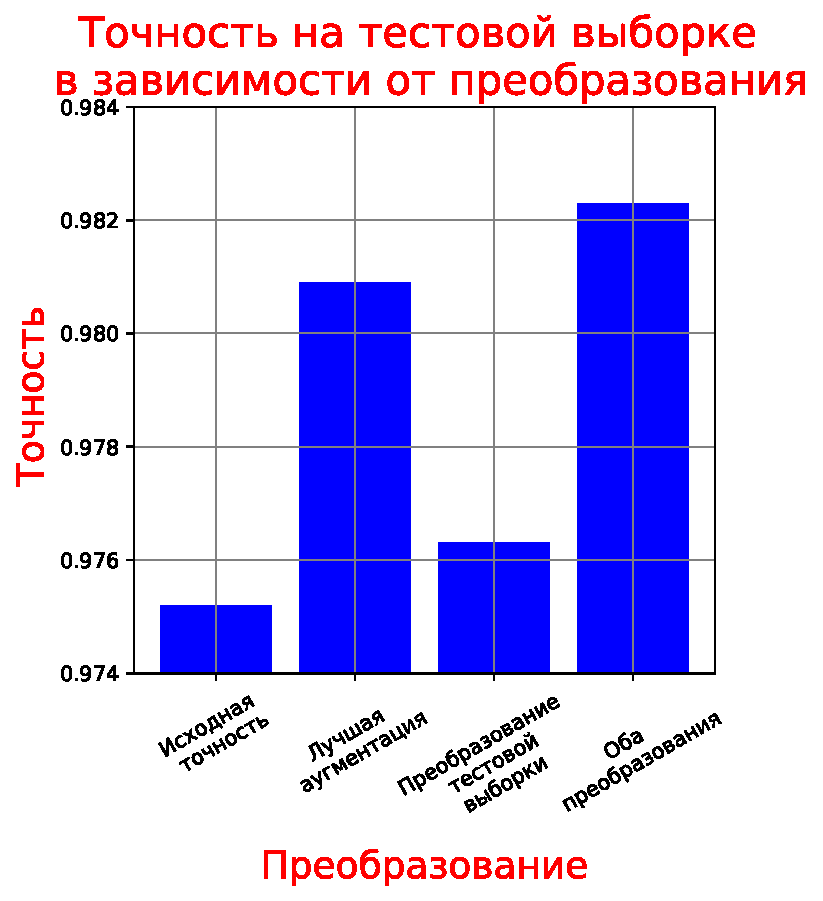
\includegraphics[width=5cm]{TASK1 PRAC сравнение.pdf}
    \end{center}
    
    А также полученный результат визуализирован с помощью матрицы ошибок ниже.
    \begin{center}
        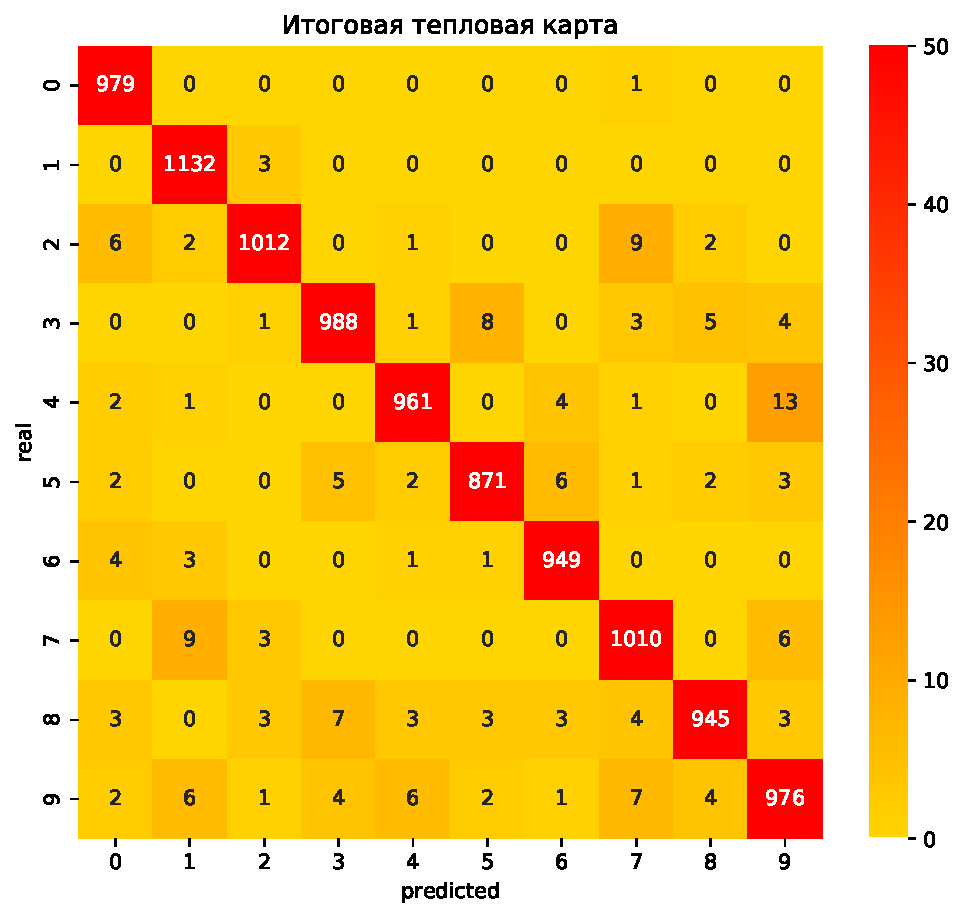
\includegraphics[width=5cm]{TASK1 end.pdf}
    \end{center}
    
Можно заметить, что теперь нет цифр, которые заметно чаще распознаются неправильно (как было ранее с "4"{ }и "9").
\end{itemize}


\subsection{Выводы}

При аугментации точность при почти любых преобразованиях повышается, прежде всего за счет увеличения обучающей выборки, но при этом значительно увеличивается время выполнения программы. На обучающей выборке исходного объема (60 тыс. изображений) время поиска ответов на стандартной тестовой выборке равно 50 секундам. При увеличении выборки в 4 раза время увеличивается до 183 секунд. При преобразовании объектов тестовой выборки улучшение достигается только в некоторых случаях путем комбинаций различных преобразований и принятия решения голосованием, но программа выполняется быстро, так как объем обучающей выборки не изменяется. 


\section{Выводы}

В данном исследовании лучшее значение доли правильно предсказанных ответов на тестовой выборке равно 0.9823. Такая точность достигнута при использовании метода brute с весами с голосом объекта $\frac{1}{distance + \epsilon}$, где $\epsilon={10}^{-5}$, и числом соседей k=4, а также совместном преобразовании объектов обучающей и тестовой выборки. При преобразовании обучающей выборки исходная выборка была увеличена в 4 раза и первая копия была преобразована почти случайным образом, вторая с помощью (не случайного) поворота на $5^\circ$, третья с помощью поворота на $-5^\circ$. Также
ко второй и третьей выборке был применен фильтр Гаусса с дисперсией 0.5. Преобразование тестовой выборки было выполнено несколько раз путем сдвига во всевозможные стороны на 1 пиксель, поворота в обе стороны на $5^\circ$, а решение было принято среди полученных ответов путем голосования. Точность метода без преобразований была равна 0.9752.

\newpage
\section*{Приложение}
\addcontentsline{toc}{section}{Приложение}

\begin{figure}[H]	
	\subfigure
	{
	    \begin{minipage}{8cm}
            \centering
            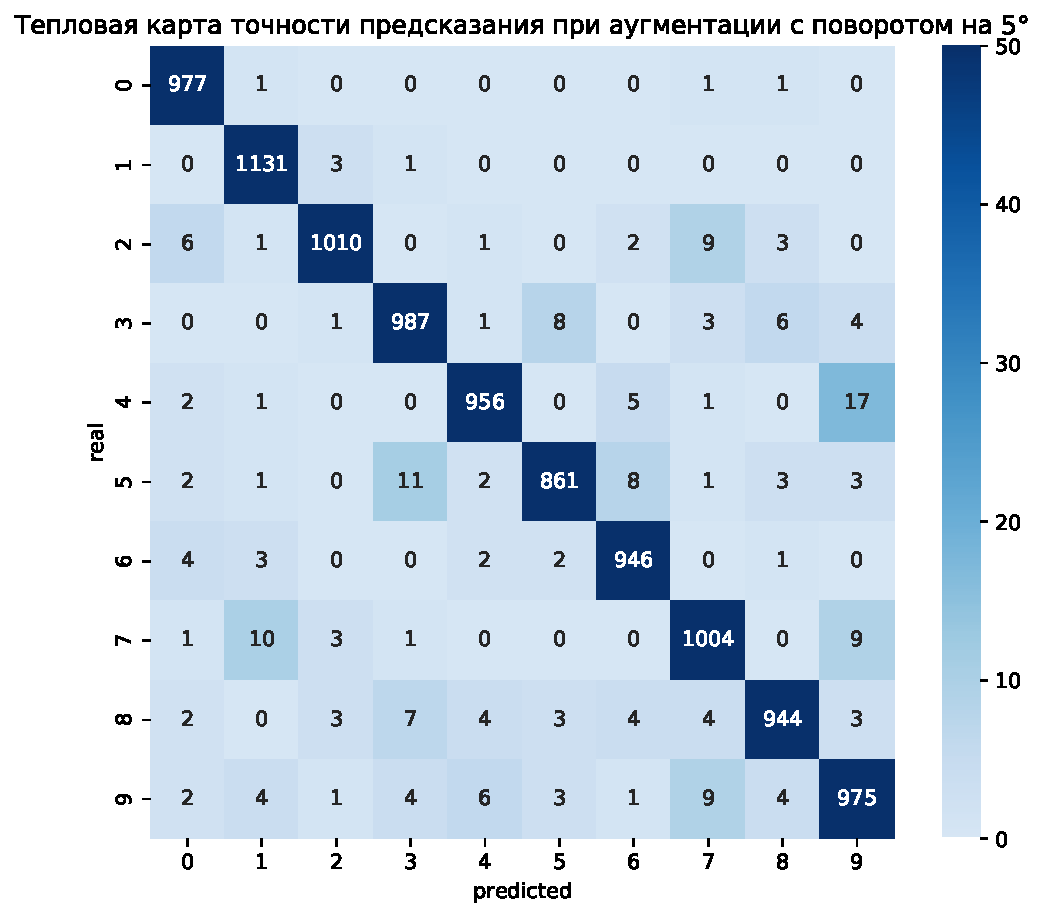
\includegraphics[scale=0.35]{TASK1 warm map rotated5.pdf}
            % \caption{Caption}
        \end{minipage}
        \label{app:rot5}
	}
	\subfigure
	{
		\begin{minipage}{8cm}
			\centering
			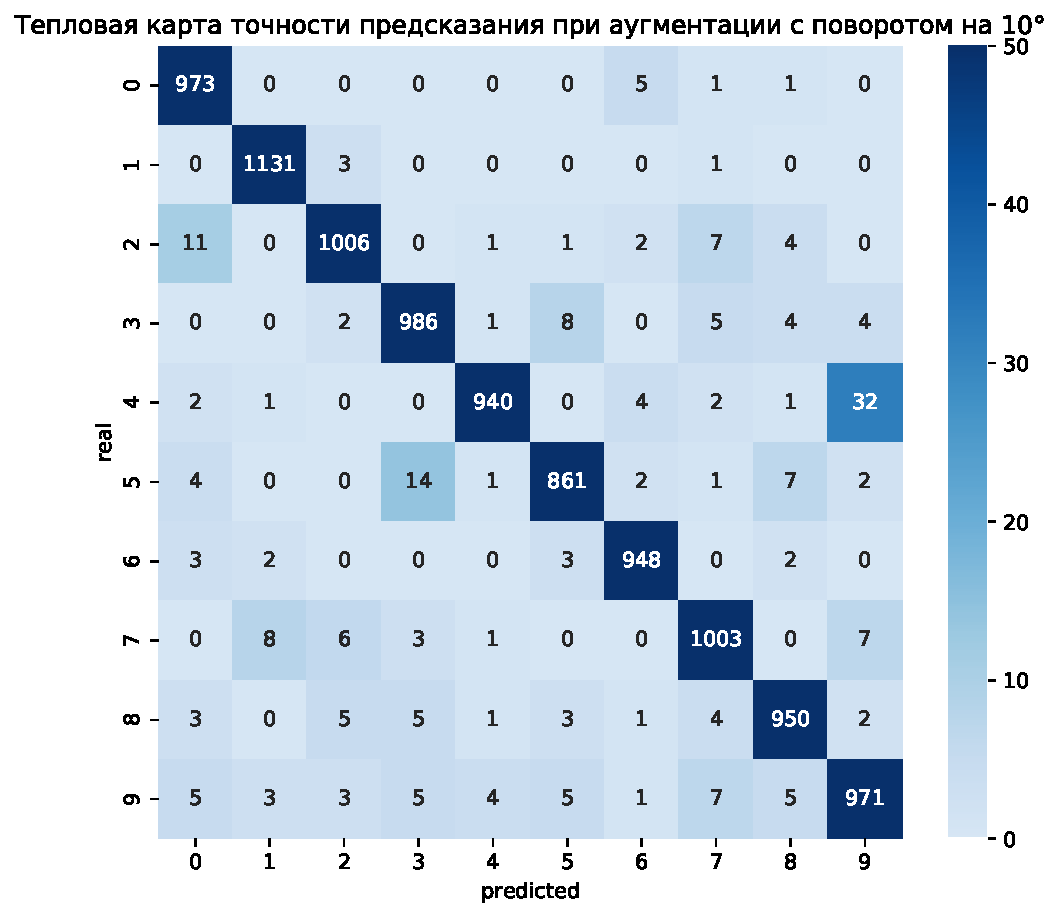
\includegraphics[scale=0.35]{TASK1 warm map rotated10.pdf}
			% \caption{Caption}
		\end{minipage}
		\label{app:rot10}
	}
	\subfigure
	{
		\begin{minipage}{8cm}
			\centering
			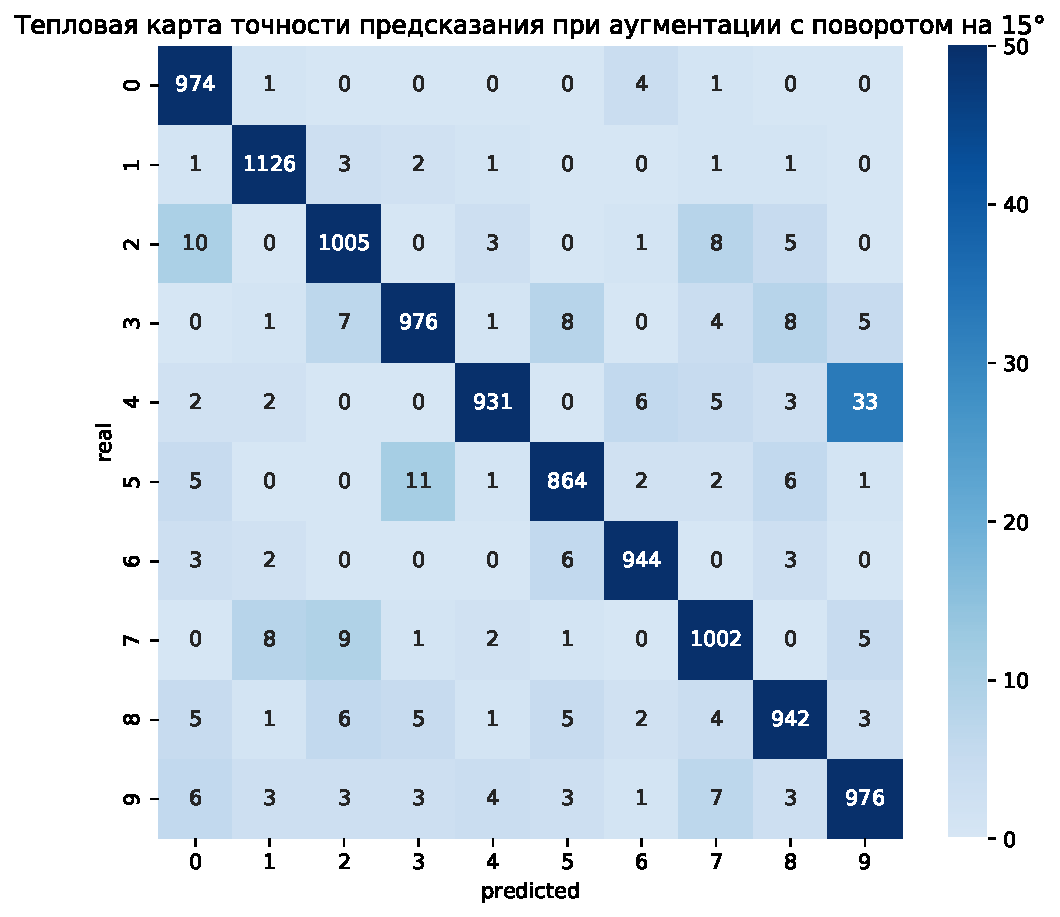
\includegraphics[scale=0.35]{TASK1 warm map rotated15.pdf}
			% \caption{Caption}
		\end{minipage}
		\label{app:rot15}
	}
	\subfigure
	{
	    \begin{minipage}{8cm}
            \centering
            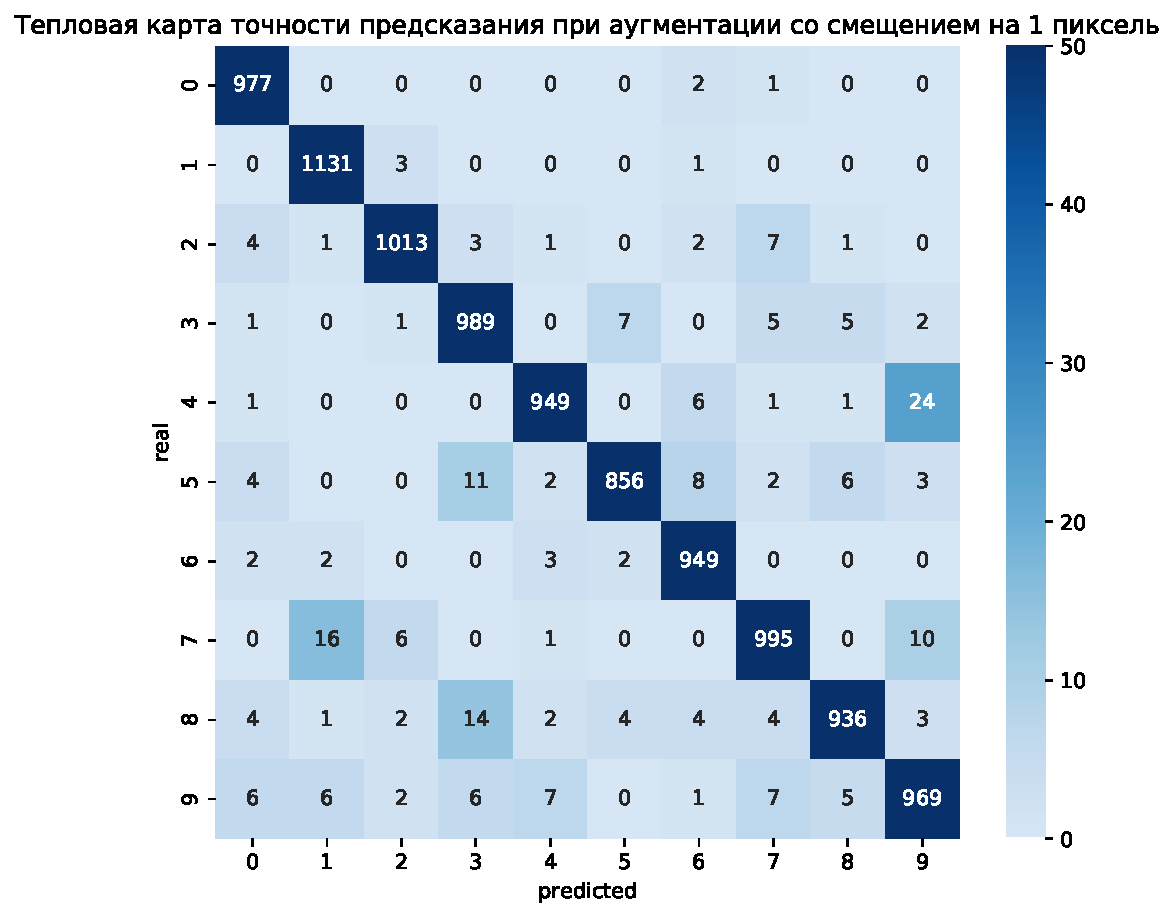
\includegraphics[scale=0.35]{TASK1 warm map shift1piks.pdf}
            % \caption{Caption}
        \end{minipage}
        \label{app:shift1}
	}
	\subfigure
	{
		\begin{minipage}{8cm}
			\centering
			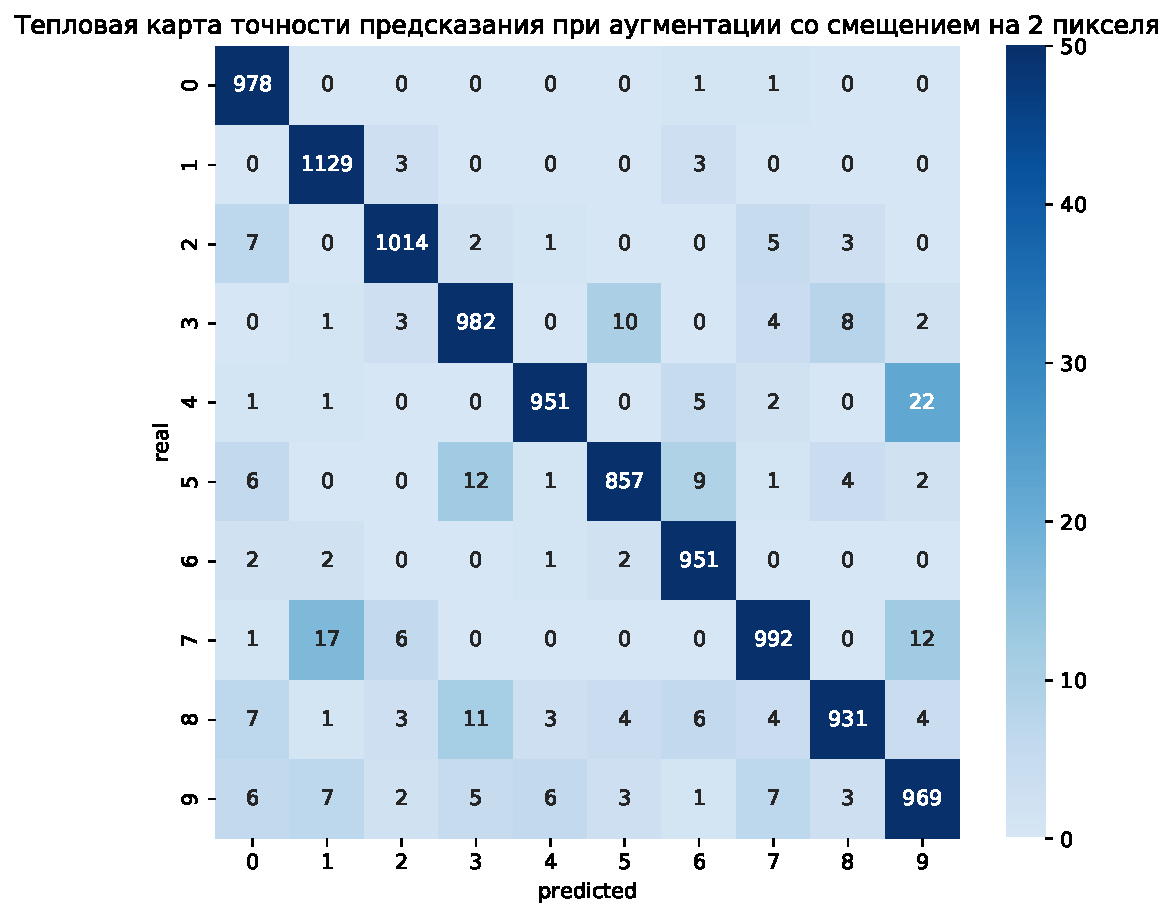
\includegraphics[scale=0.35]{TASK1 warm map shift2piks.pdf}
			% \caption{Caption}
		\end{minipage}
		\label{app:shift2}
	}
	\subfigure
	{
		\begin{minipage}{8cm}
			\centering
			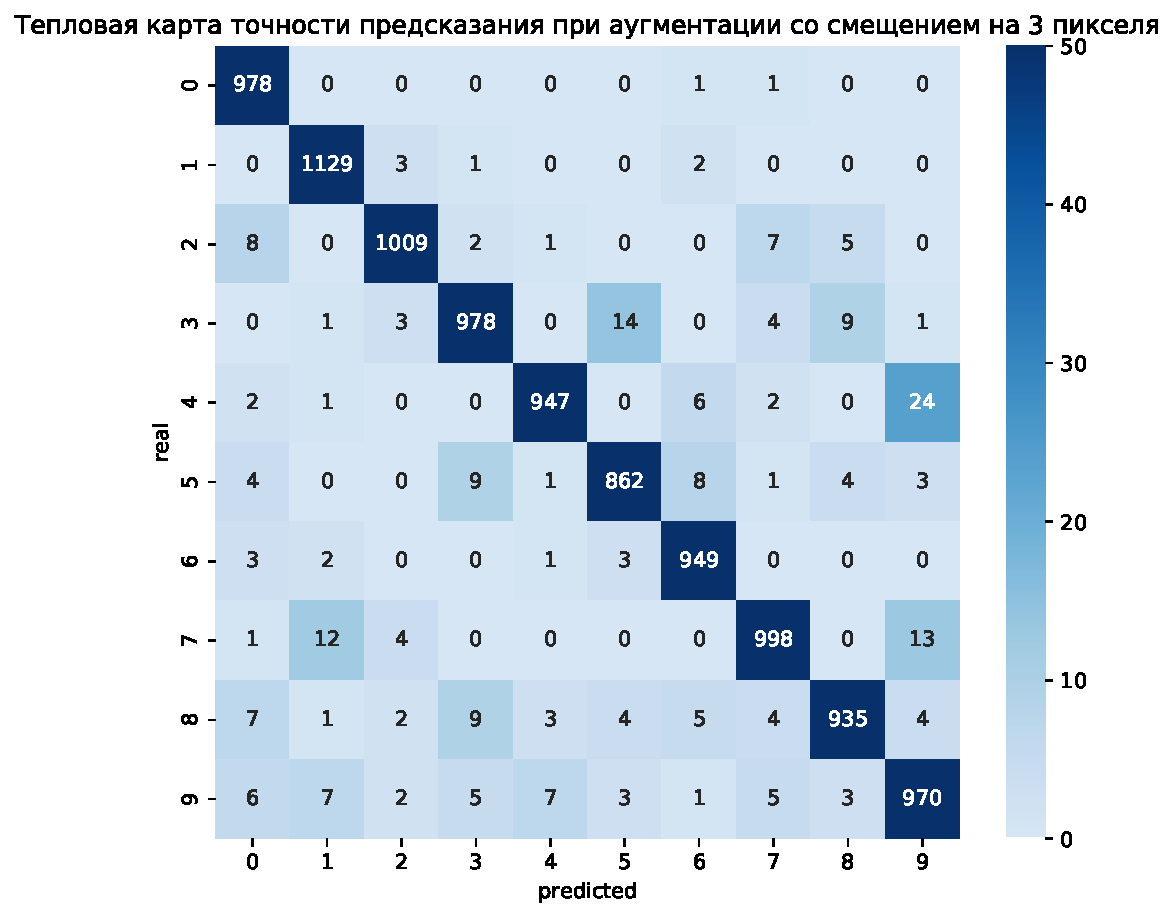
\includegraphics[scale=0.35]{TASK1 warm map shift3piks.pdf}
			% \caption{Caption}
		\end{minipage}
		\label{app:shift3}
	}
	% \caption{Caption}
\end{figure}


\newpage
\begin{figure}[H]	
	\subfigure
	{
        \begin{minipage}{8cm}
            \centering
            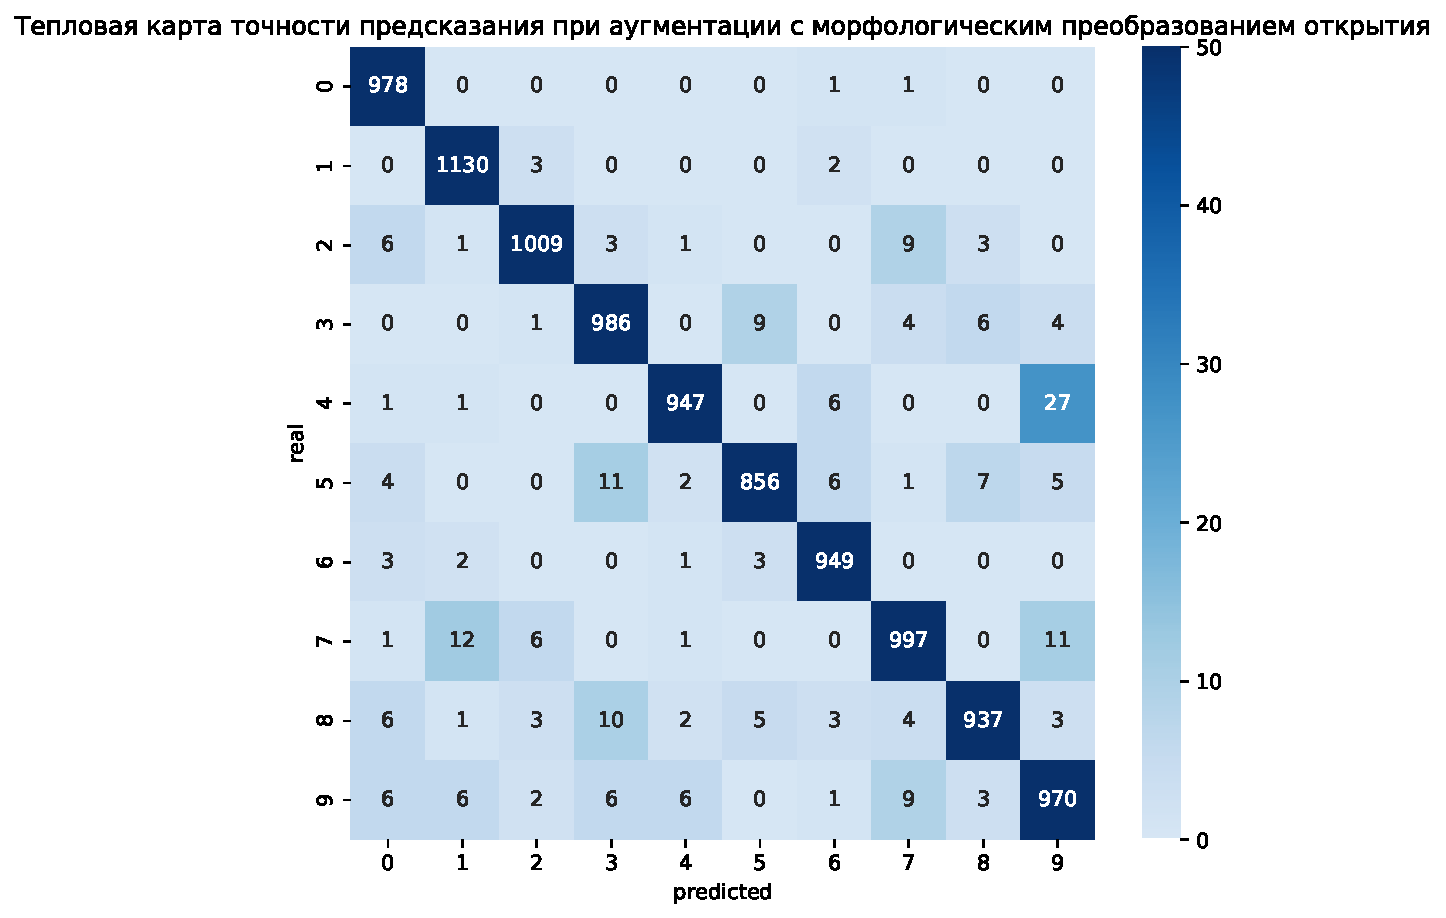
\includegraphics[scale=0.33]{TASK1 warm map open.pdf}
            % \caption{Caption}
        \end{minipage}
        \label{app:open}
	}
	\subfigure
	{
		\begin{minipage}{8cm}
			\centering
			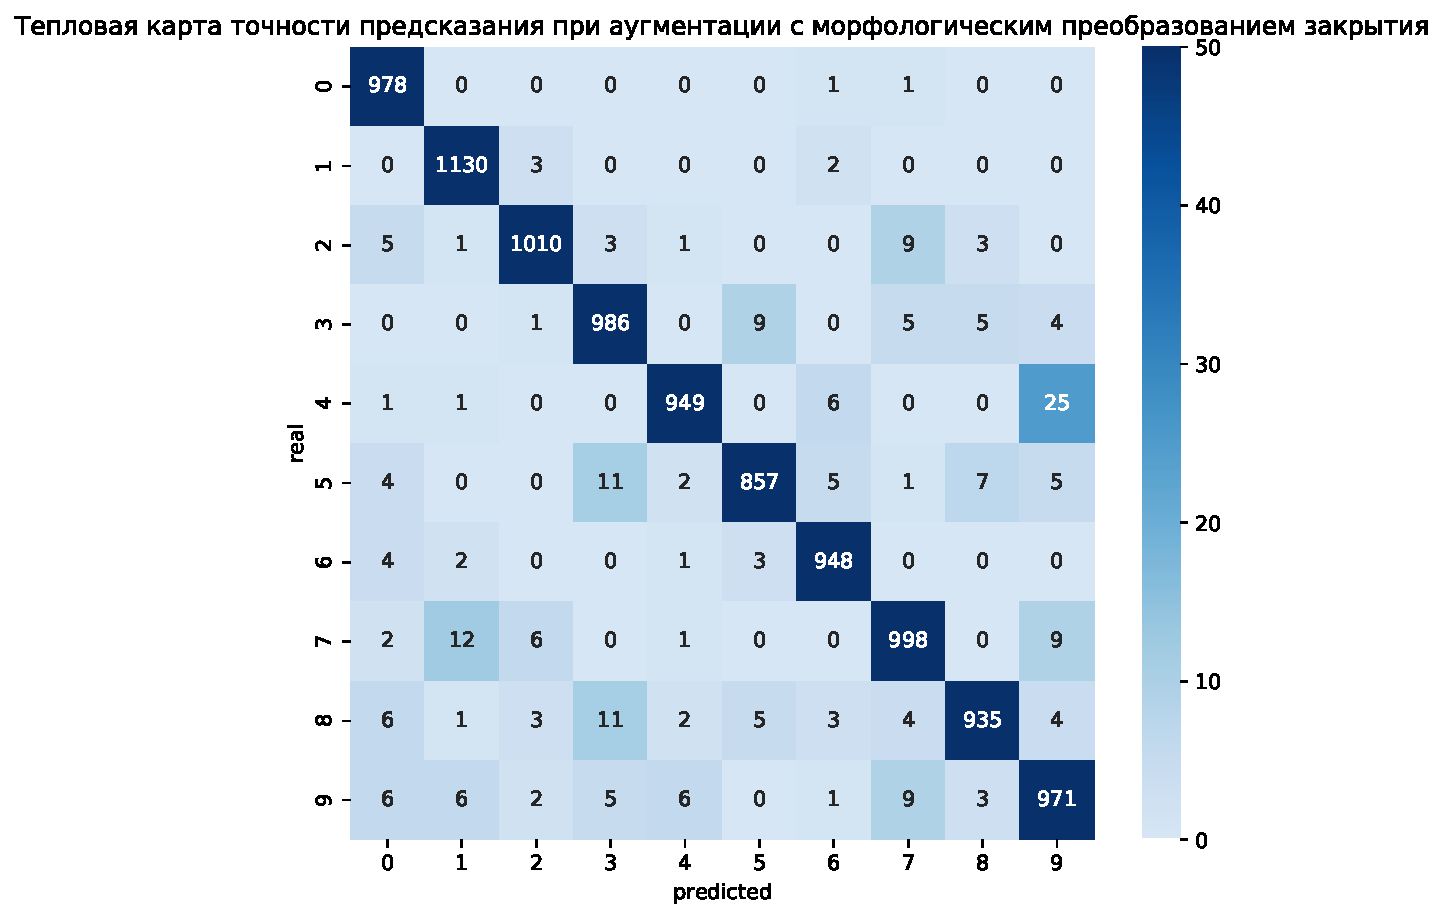
\includegraphics[scale=0.33]{TASK1 warm map close.pdf}
			% \caption{Caption}
		\end{minipage}
		\label{app:close}
	}
	\subfigure
	{
		\begin{minipage}{8cm}
			\centering
			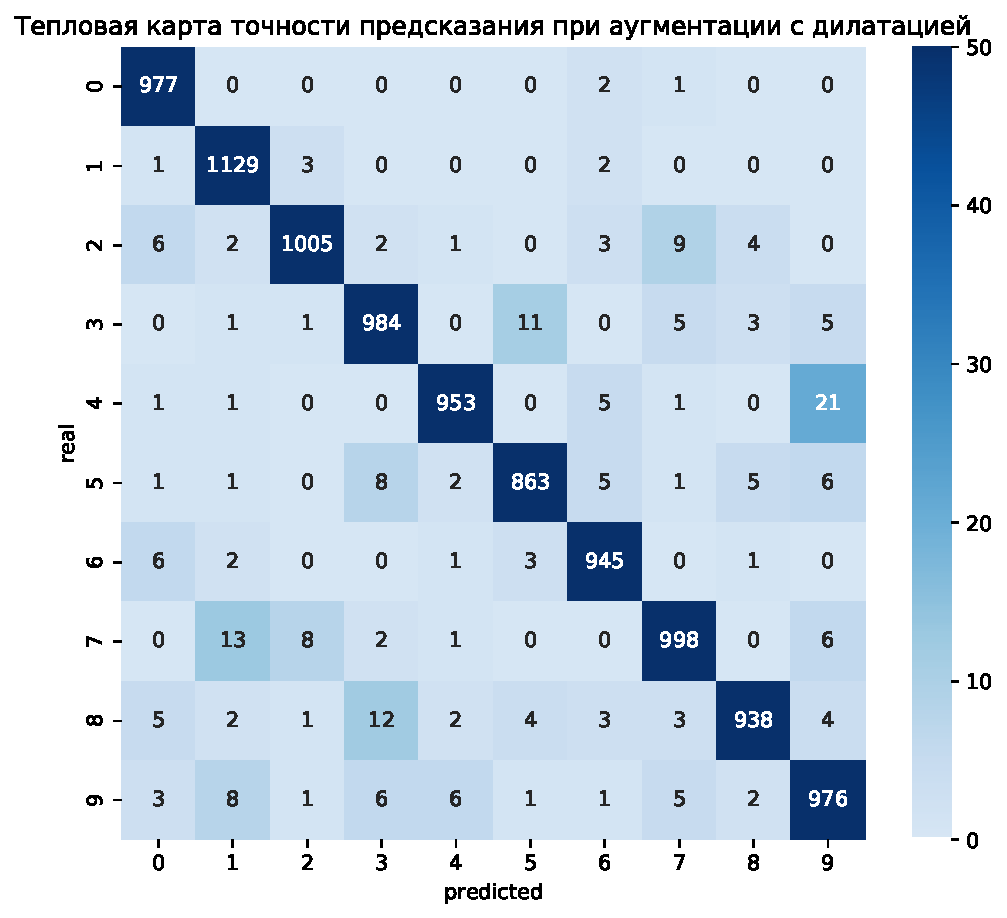
\includegraphics[scale=0.35]{TASK1 warm map dilate.pdf}
		\end{minipage}
		\label{app:dilate}
	}
	\subfigure
	{
		\begin{minipage}{8cm}
			\centering
			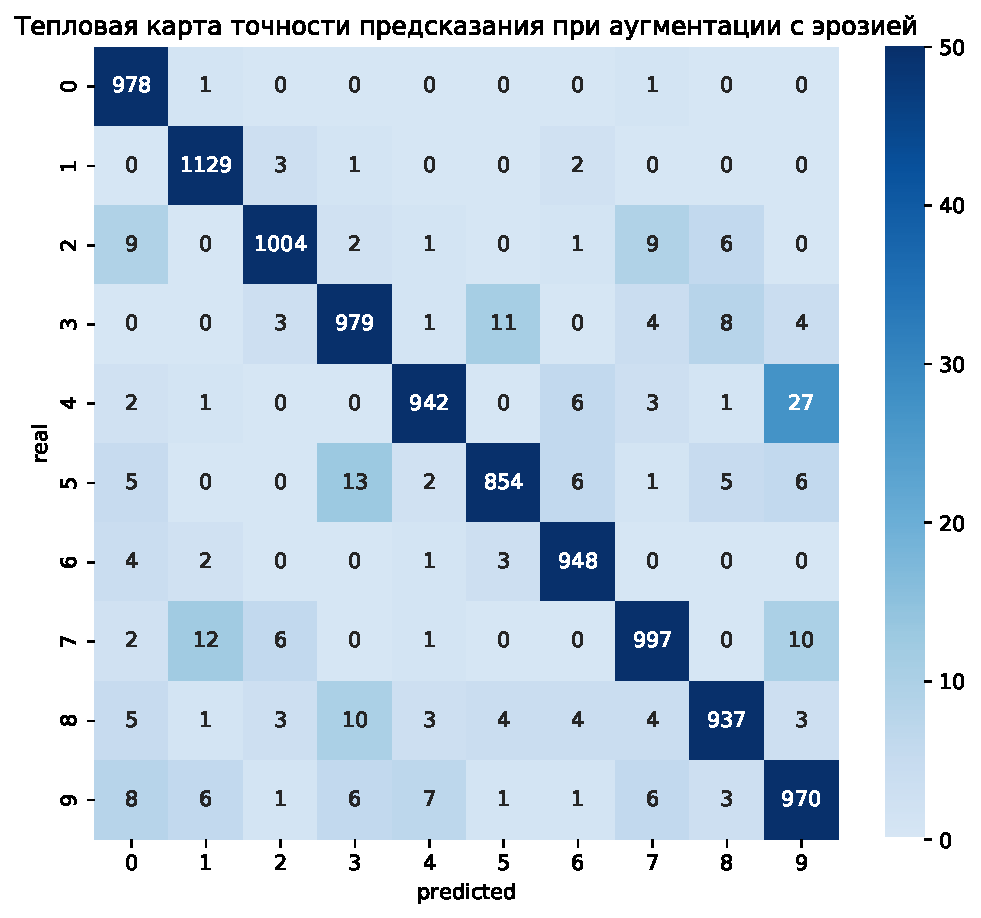
\includegraphics[scale=0.35]{TASK1 warm map erode.pdf}
			% \caption{Caption}
		\end{minipage}
		\label{app:erode}
	}
	\subfigure
	{
	    \begin{minipage}{8cm}
	        \centering
	        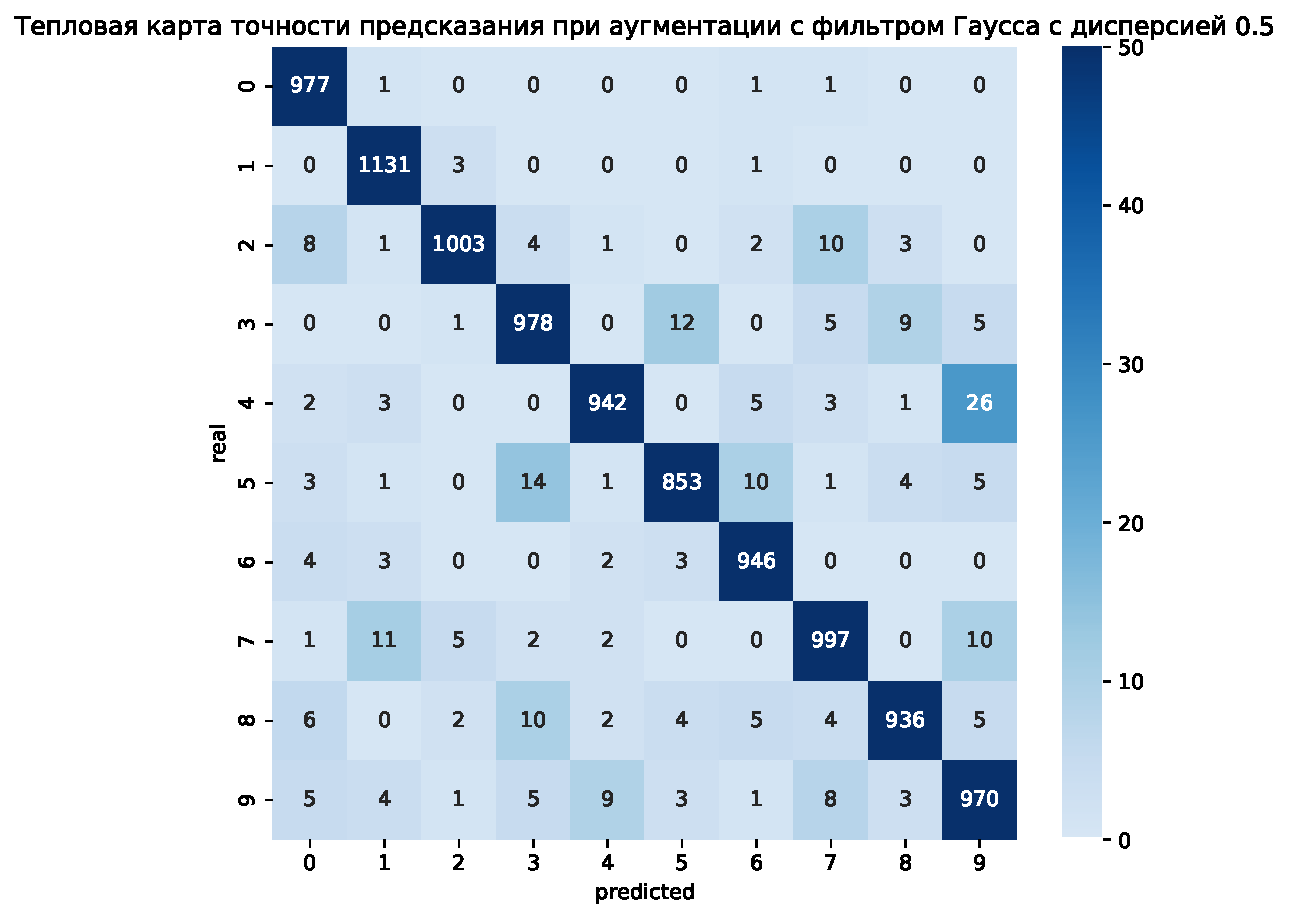
\includegraphics[scale=0.35]{TASK1 warm map filter0_5.pdf}
	        % \caption{Caption}
	    \end{minipage}
	    \label{app:filter0_5}
	}
	\subfigure
	{
		\begin{minipage}{8cm}
			\centering
			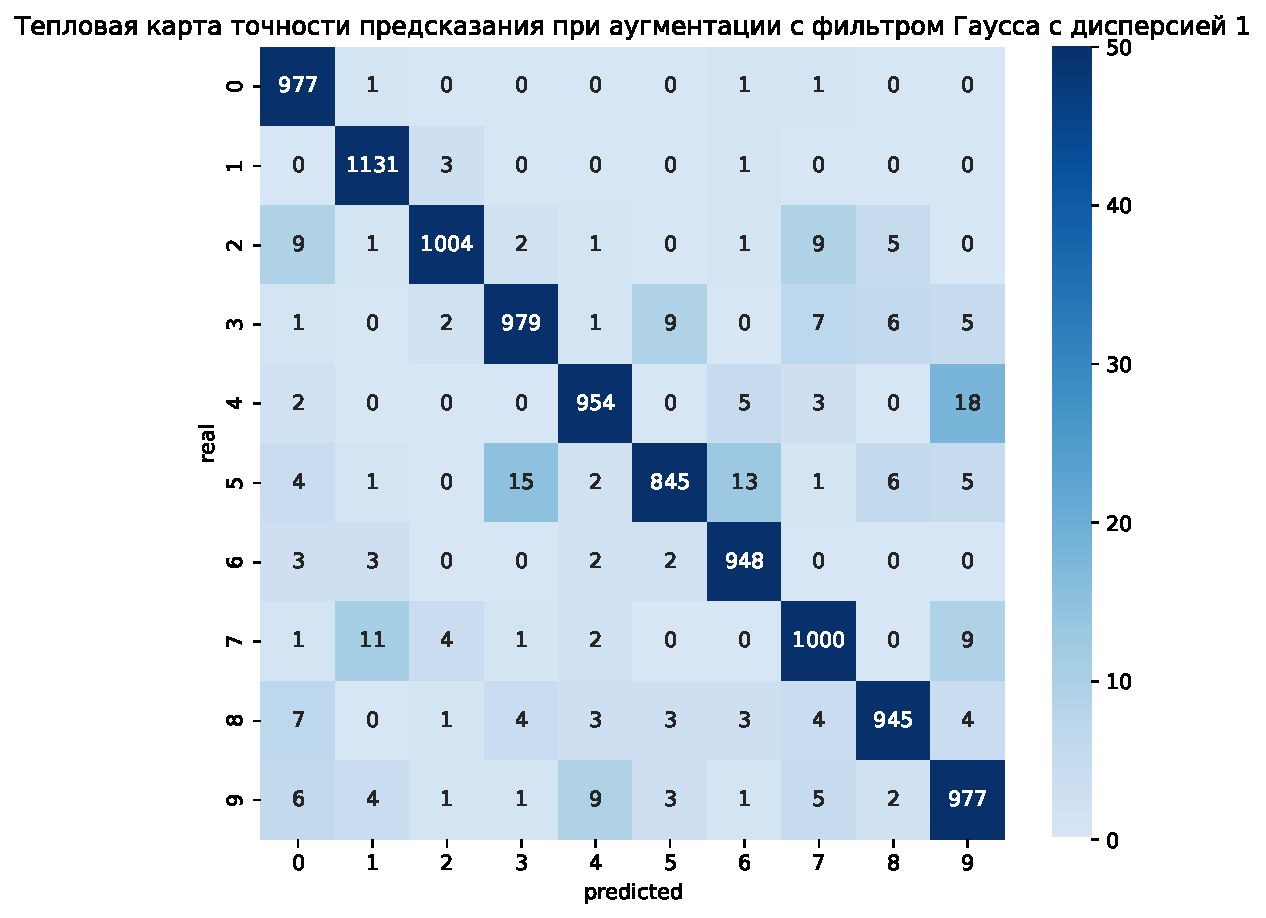
\includegraphics[scale=0.35]{TASK1 warm map filter1.pdf}
			% \caption{Caption}
		\end{minipage}
		\label{app:filter1}
	}
	% \caption{Caption}
\end{figure}


\newpage
\begin{figure}[h]
	\subfigure
	{
		\begin{minipage}{8cm}
			\centering
			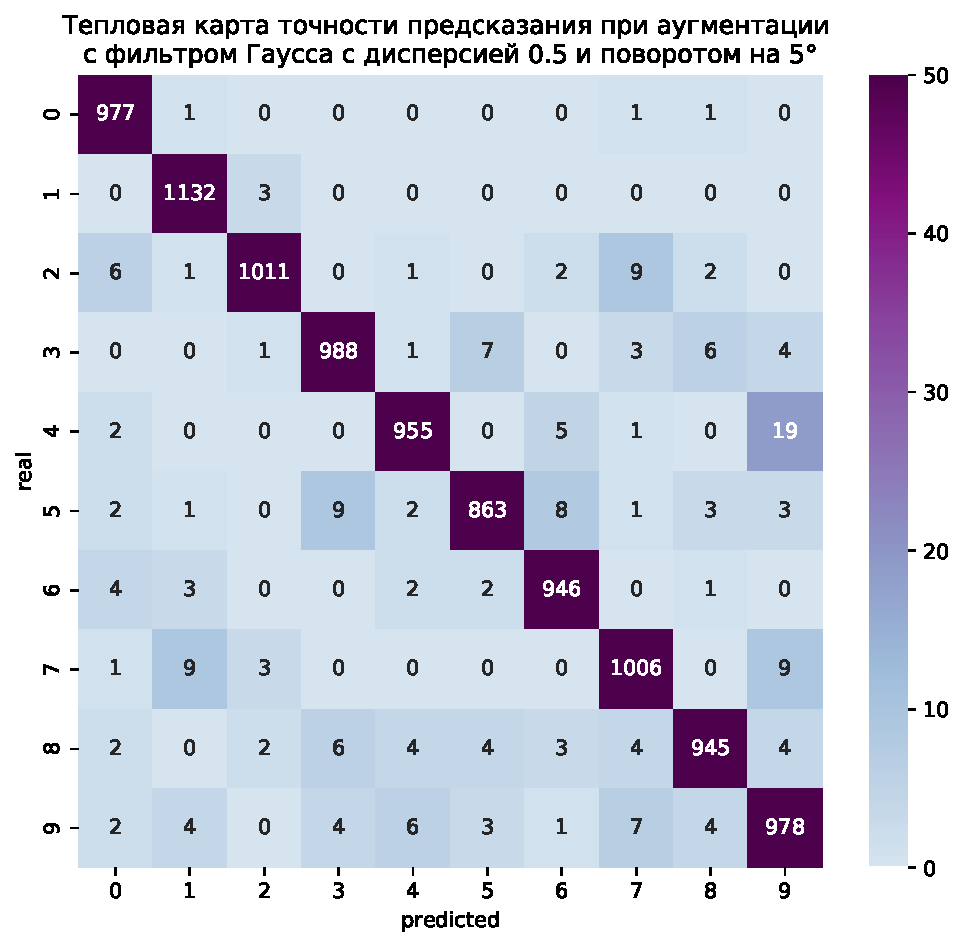
\includegraphics[scale=0.35]{TASK1 warm map 0.pdf}
			% \caption{Caption}
		\end{minipage}
		\label{app:violet0}
	}
	\subfigure
	{
		\begin{minipage}{8cm}
			\centering
			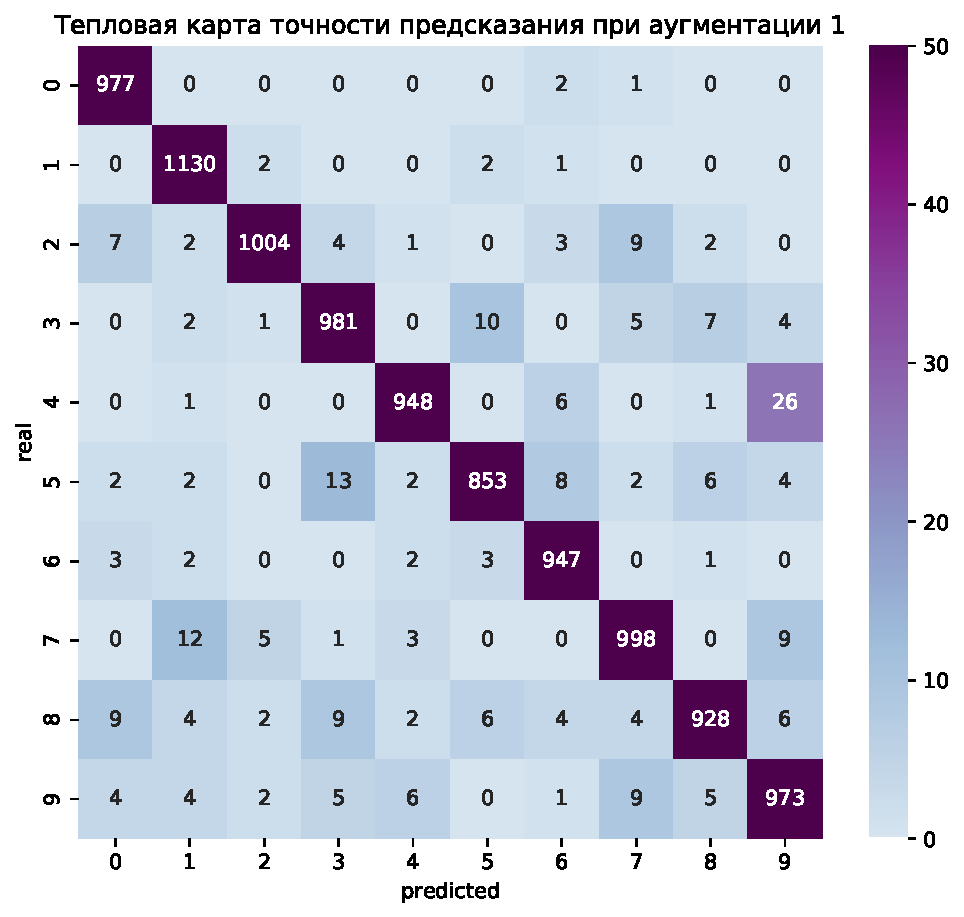
\includegraphics[scale=0.35]{TASK1 warm map 1.pdf}
			% \caption{Caption}
		\end{minipage}
		\label{app:violet1}
	}
	\subfigure
	{
		\begin{minipage}{8cm}
			\centering
			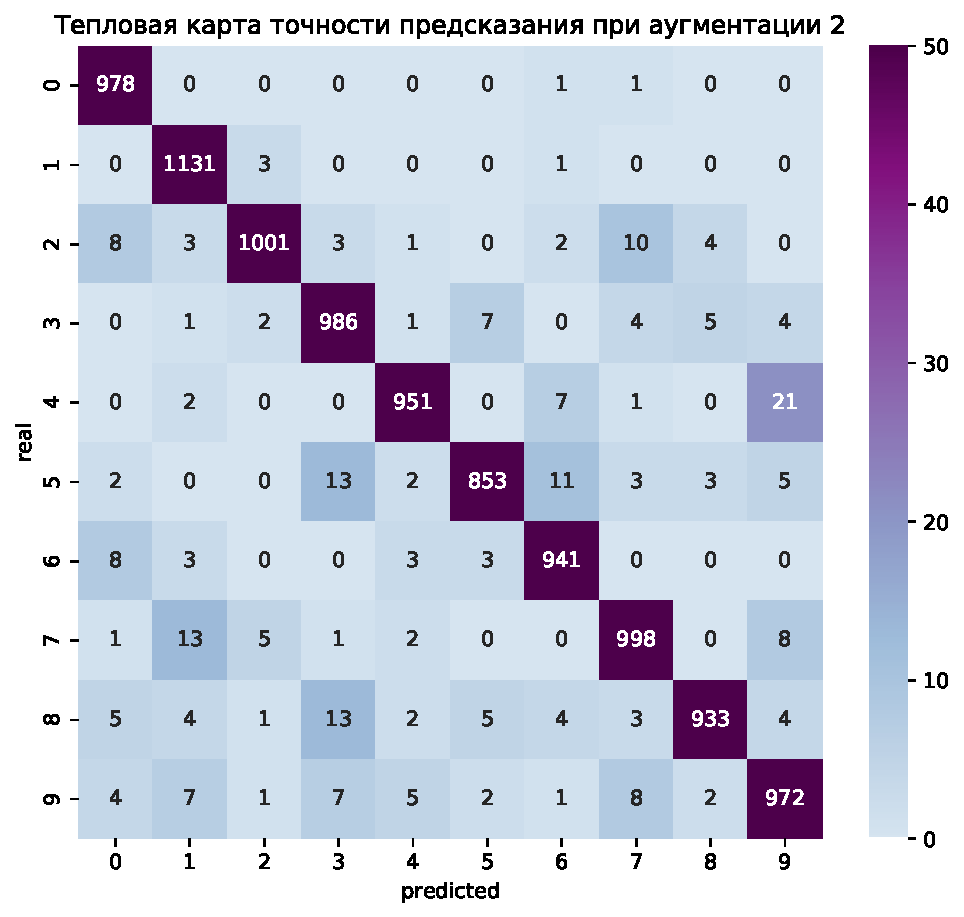
\includegraphics[scale=0.35]{TASK1 warm map 2.pdf}
			% \caption{Caption}
		\end{minipage}
		\label{app:violet2}
	}
	\subfigure
	{
        \begin{minipage}{8cm}
            \centering
            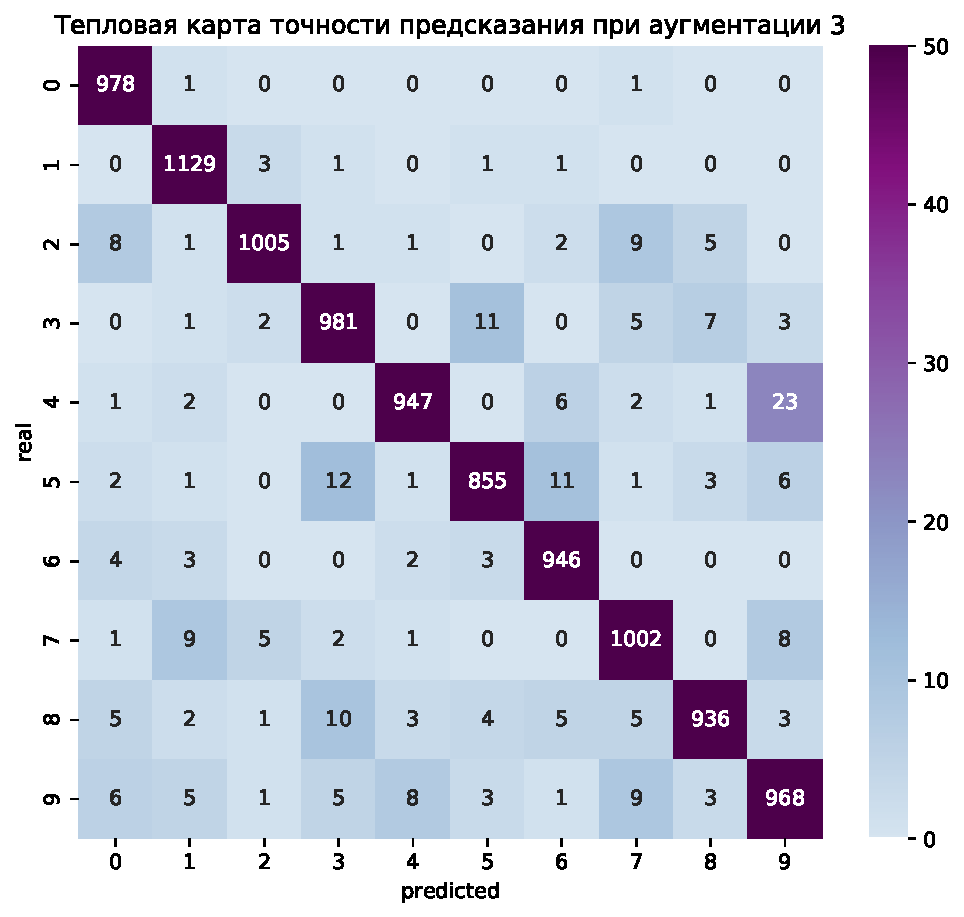
\includegraphics[scale=0.35]{TASK1 warm map 3.pdf}
            % \caption{Caption}
		\end{minipage}
		\label{app:violet3}
	}
	\subfigure
	{
        \begin{minipage}{8cm}
            \centering
            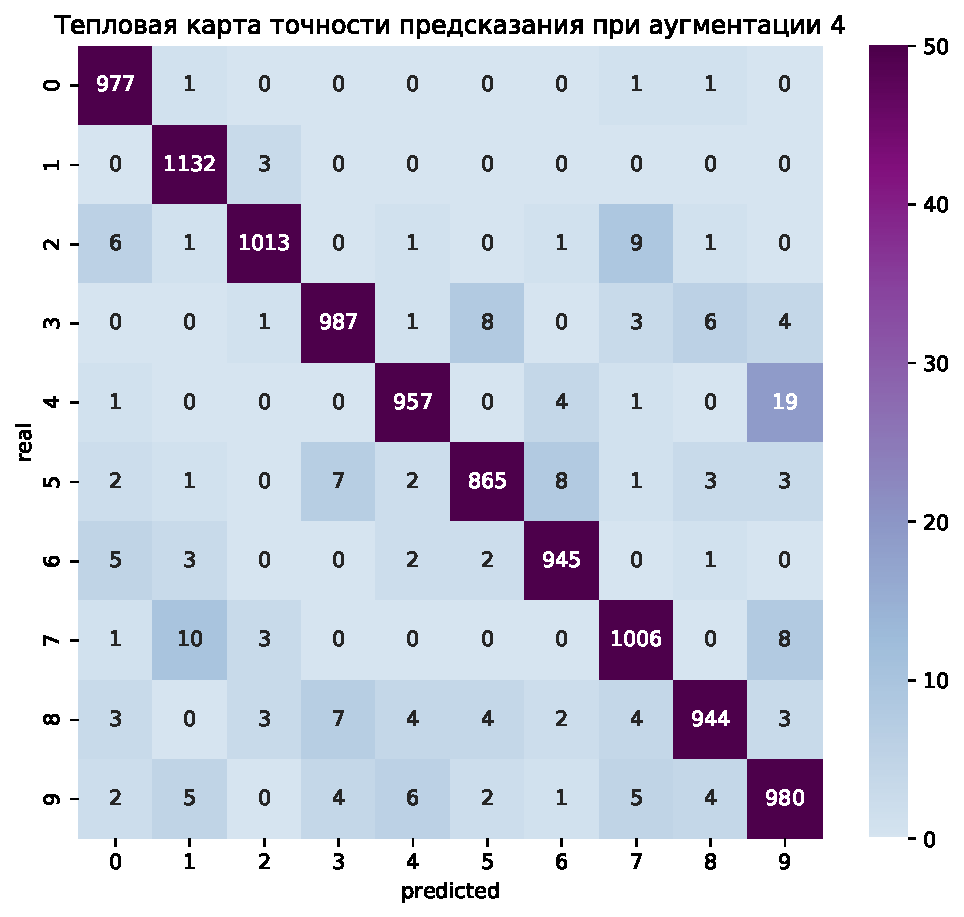
\includegraphics[scale=0.35]{TASK1 warm map 4.pdf}
            % \caption{Caption}
		\end{minipage}
		\label{app:violet4}
	}
	\captionsetup{labelformat=empty, labelsep=none}
	\caption{ }
\end{figure}

\newpage
\begin{figure}[h]	
	\subfigure
	{
        \begin{minipage}{8cm}
            \centering
            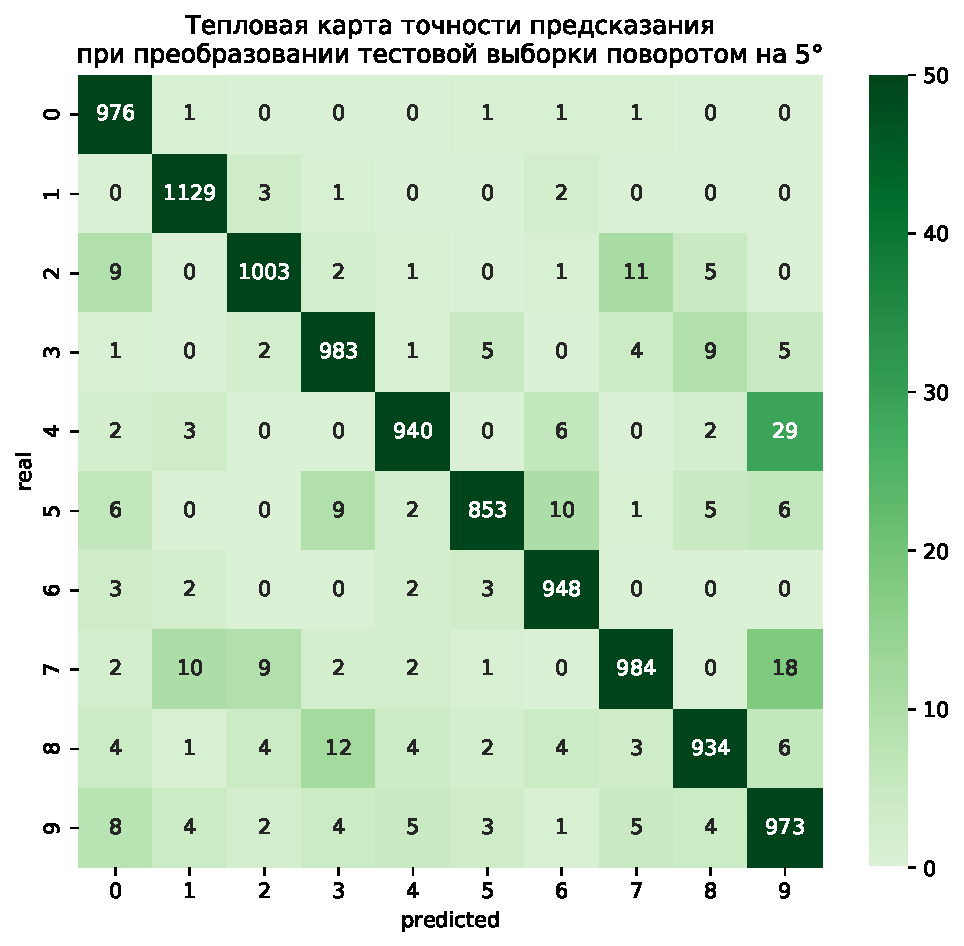
\includegraphics[scale=0.33]{TASK1 test rotated5.pdf}
            % \caption{Caption}
        \end{minipage}
        \label{app6:rot5}
	}
	\subfigure
	{
		\begin{minipage}{8cm}
			\centering
			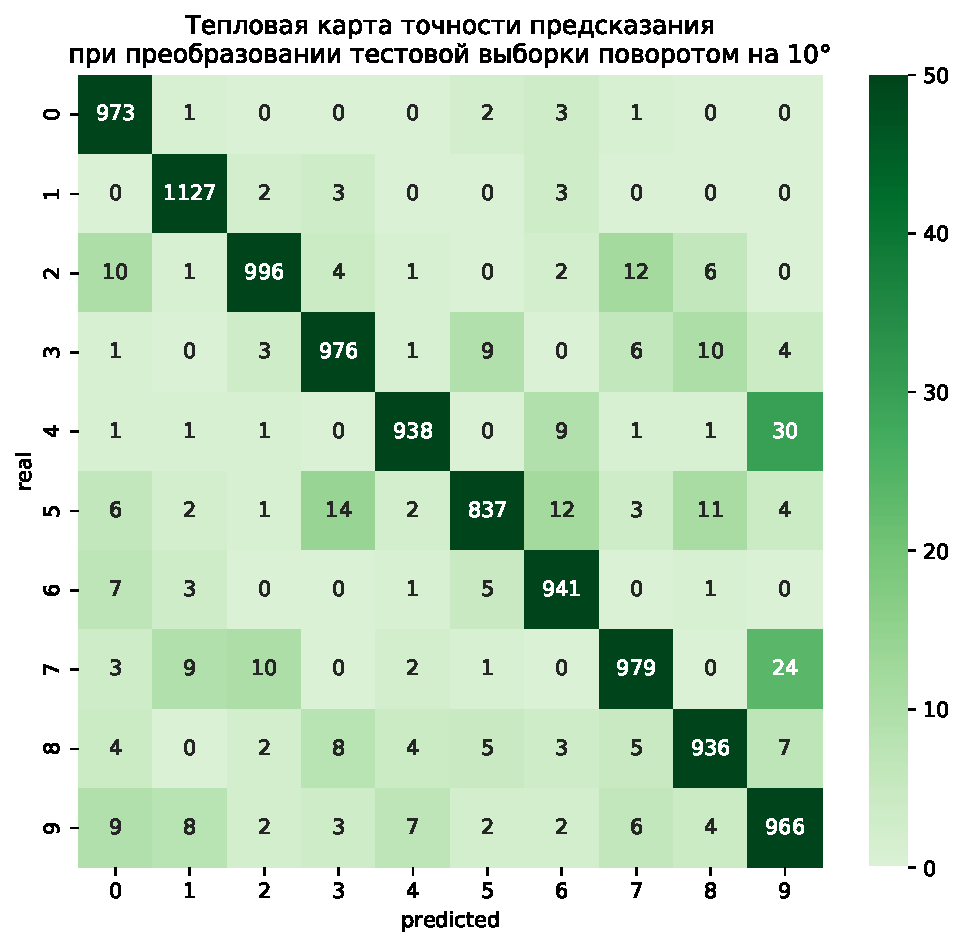
\includegraphics[scale=0.33]{TASK1 test rotated10.pdf}
			% \caption{Caption}
		\end{minipage}
		\label{app6:rot10}
	}
	\subfigure
	{
		\begin{minipage}{8cm}
			\centering
			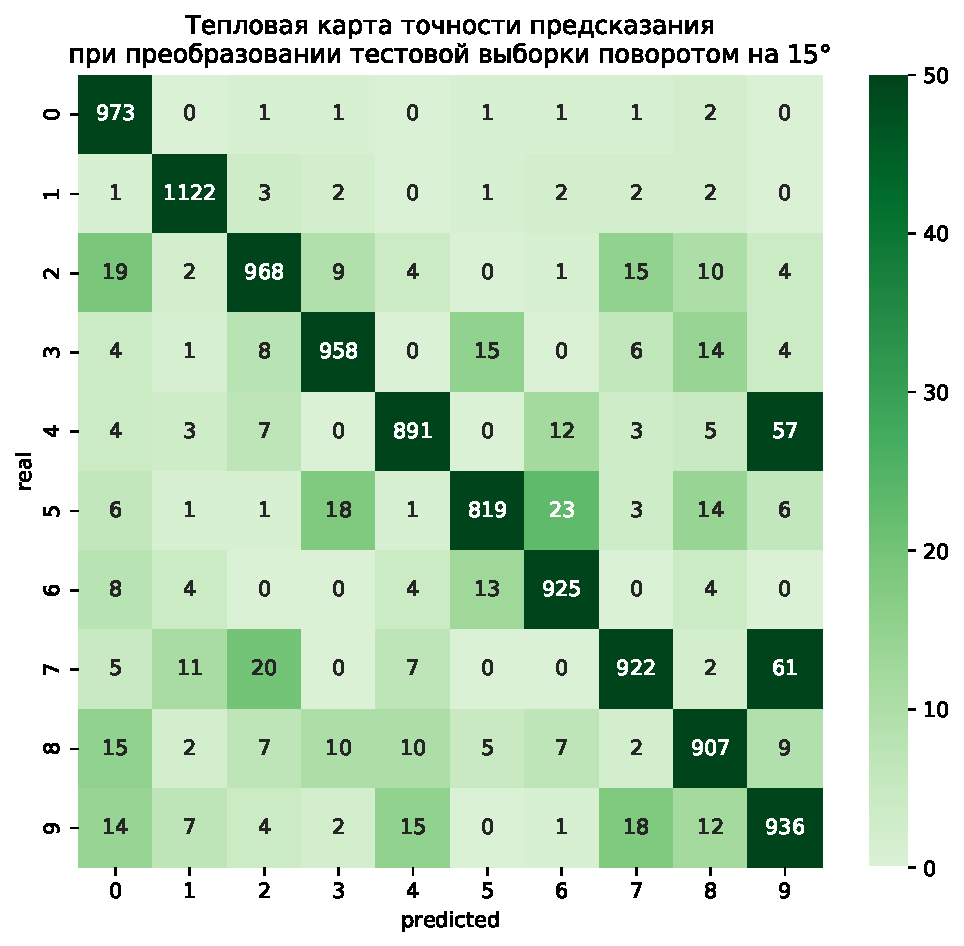
\includegraphics[scale=0.35]{TASK1 test rotated15.pdf}
		\end{minipage}
		\label{app6:rot15}
	}
	\subfigure
	{
		\begin{minipage}{8cm}
			\centering
			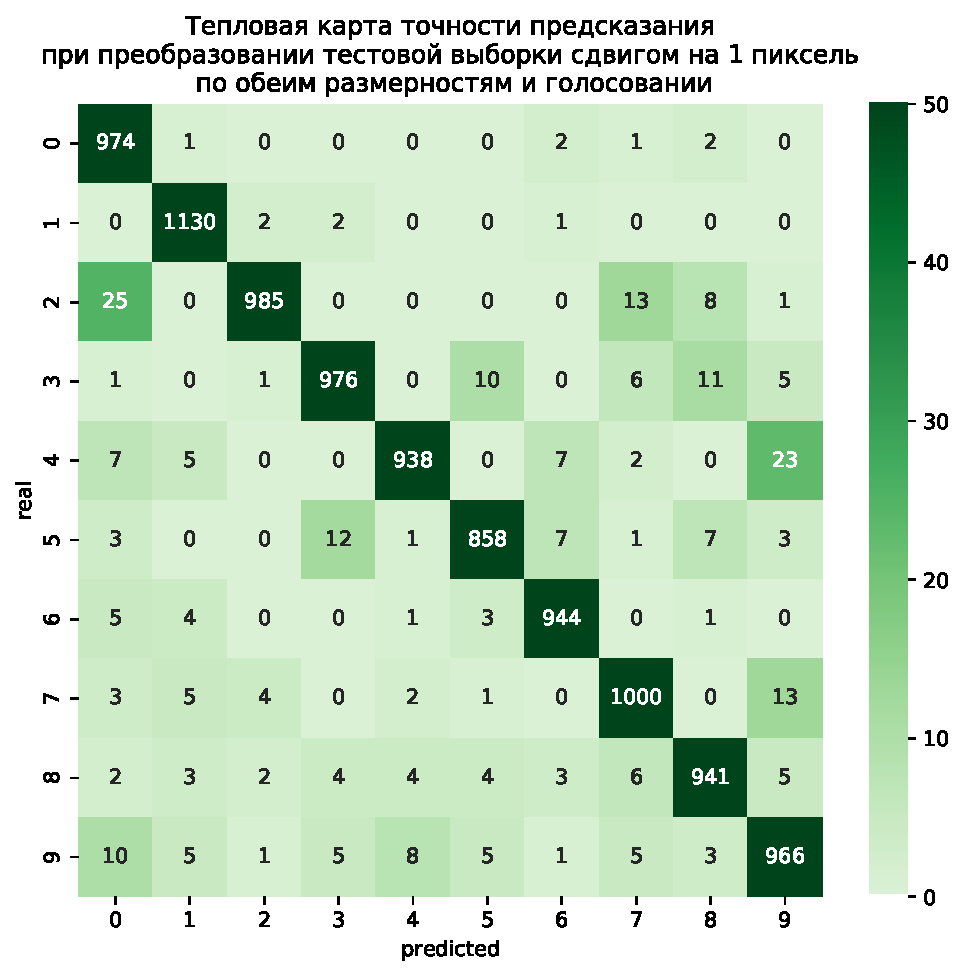
\includegraphics[scale=0.35]{TASK1 test shift 1 .pdf}
			% \caption{Caption}
		\end{minipage}
		\label{app6:shift1}
	}
	\subfigure
	{
	    \begin{minipage}{8cm}
	        \centering
	        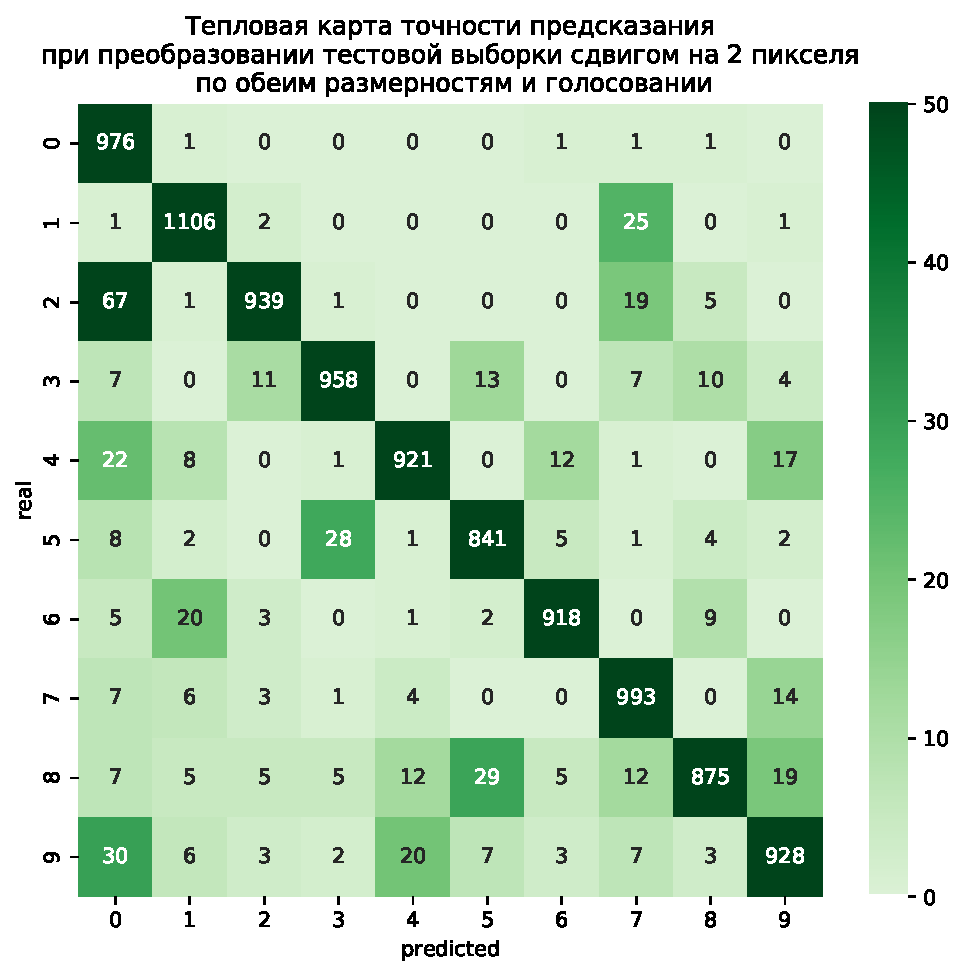
\includegraphics[scale=0.35]{TASK1 test shift 2.pdf}
	        % \caption{Caption}
	    \end{minipage}
	    \label{app6:shift2}
	}
	\subfigure
	{
		\begin{minipage}{8cm}
			\centering
			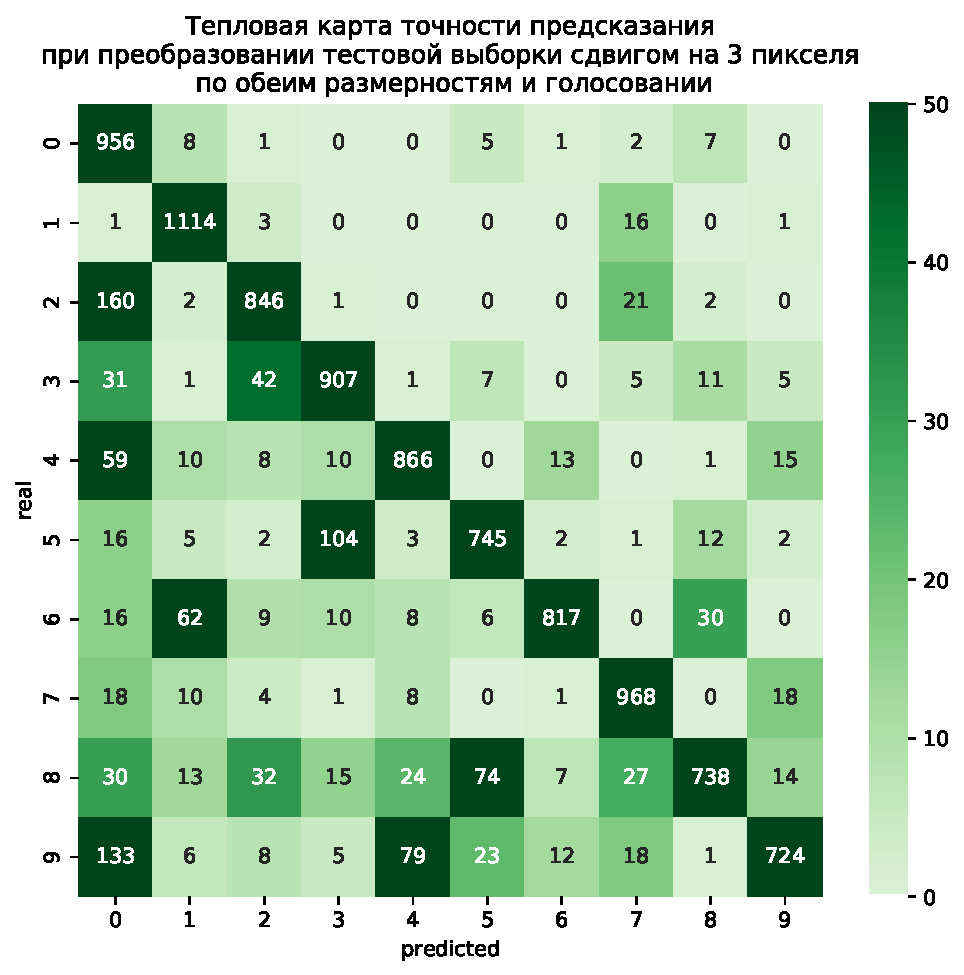
\includegraphics[scale=0.35]{TASK1 test shift 3.pdf}
			% \caption{Caption}
		\end{minipage}
		\label{app6:shift3}
	}
	% \caption{Caption}
\end{figure}

\newpage
\begin{figure}[h]	
	\subfigure
	{
	    \begin{minipage}{8cm}
	        \centering
	        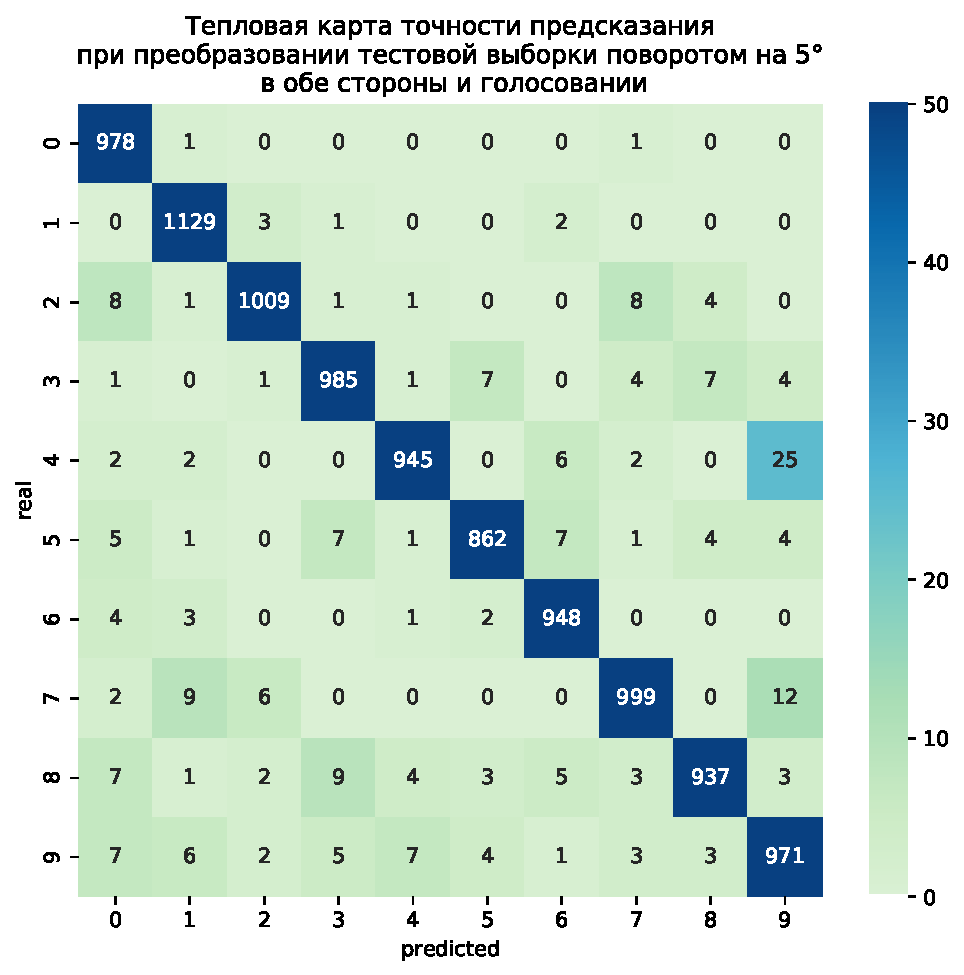
\includegraphics[scale=0.35]{TASK1 test 5 + - .pdf}
	        % \caption{Caption}
	    \end{minipage}
	    \label{app6:rot5+-}
	}
	\subfigure
	{
		\begin{minipage}{8cm}
			\centering
			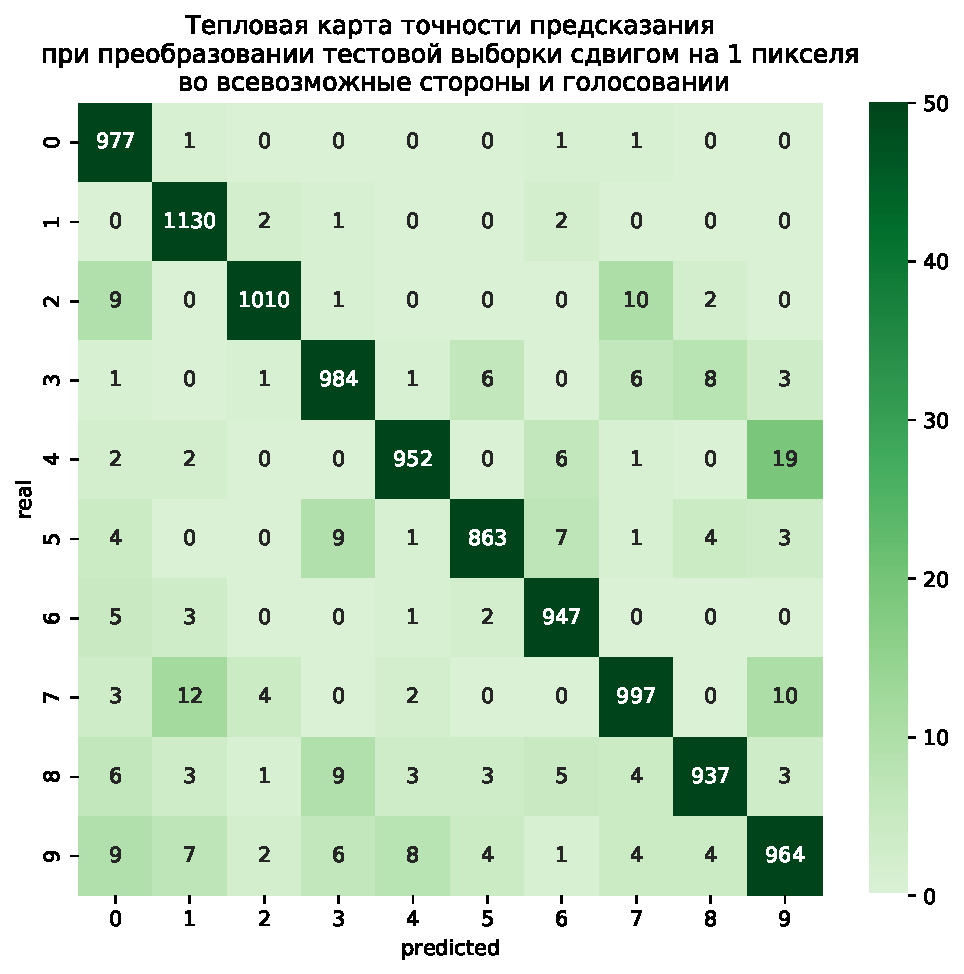
\includegraphics[scale=0.35]{TASK1 test good shift.pdf}
			% \caption{Caption}
		\end{minipage}
		\label{app6:goodshift}
	}
	\subfigure
	{
	    \begin{minipage}{8cm}
	        \centering
	        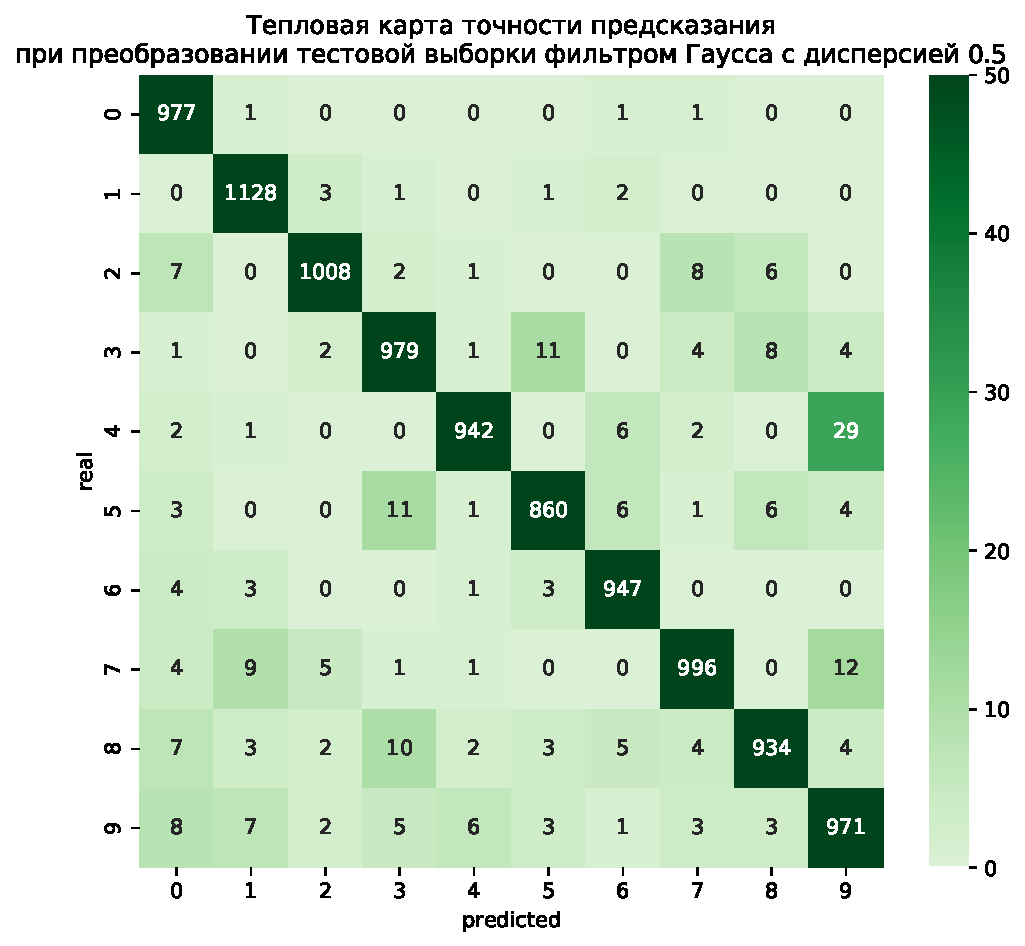
\includegraphics[scale=0.35]{TASK1 test gaus05.pdf}
	        % \caption{Caption}
	    \end{minipage}
	    \label{app6:gauss05}
	}
	\subfigure
	{
		\begin{minipage}{8cm}
			\centering
			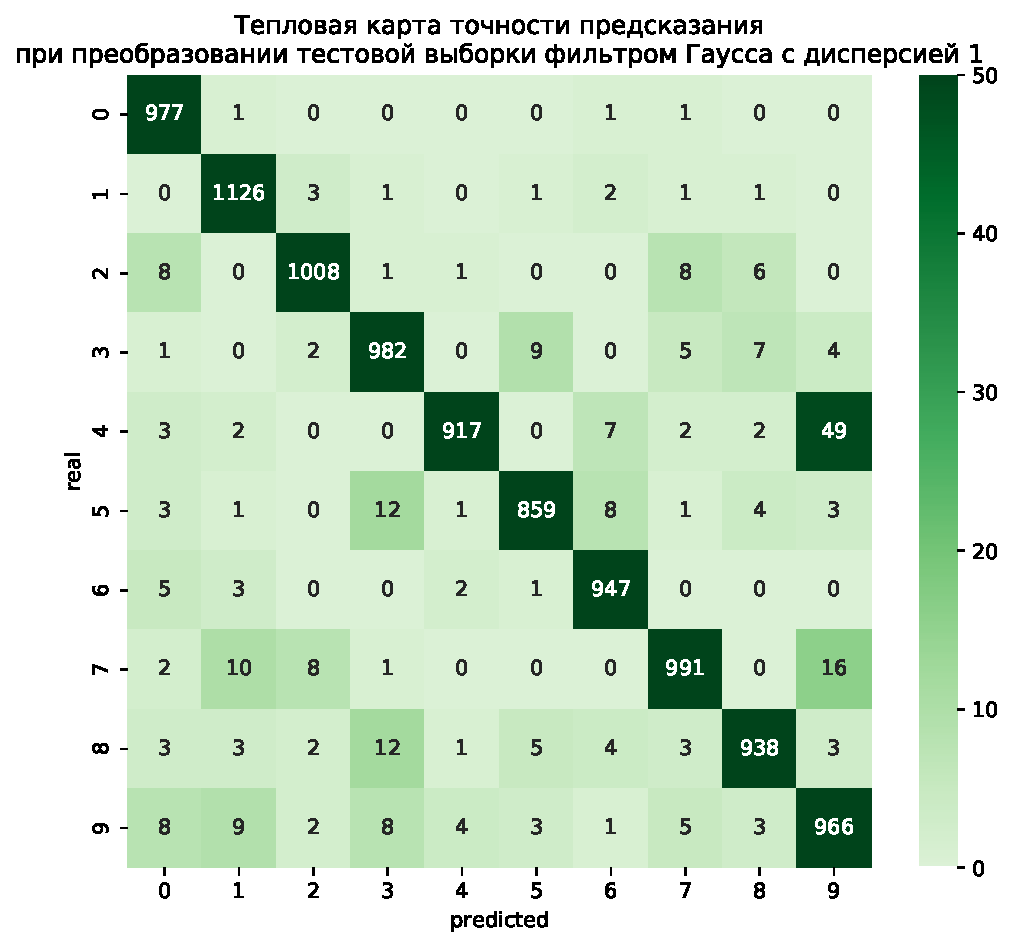
\includegraphics[scale=0.35]{TASK1 test gaus1.pdf}
			% \caption{Caption}
		\end{minipage}
		\label{app6:gauss1}
	}
	\subfigure
	{
		\begin{minipage}{8cm}
			\centering
			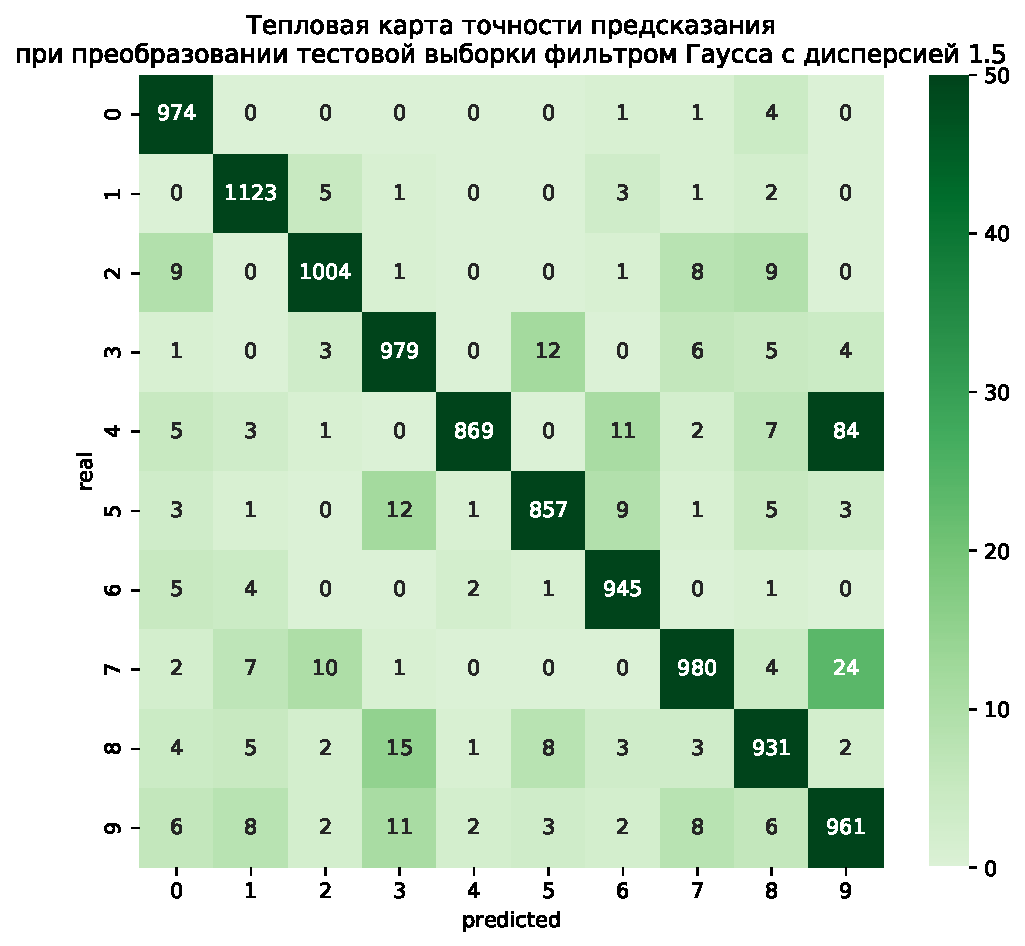
\includegraphics[scale=0.35]{TASK1 test gaus15.pdf}
			% \caption{Caption}
		\end{minipage}
		\label{app6:gauss15}
	}
	\subfigure
	{
		\begin{minipage}{8cm}
			\centering
			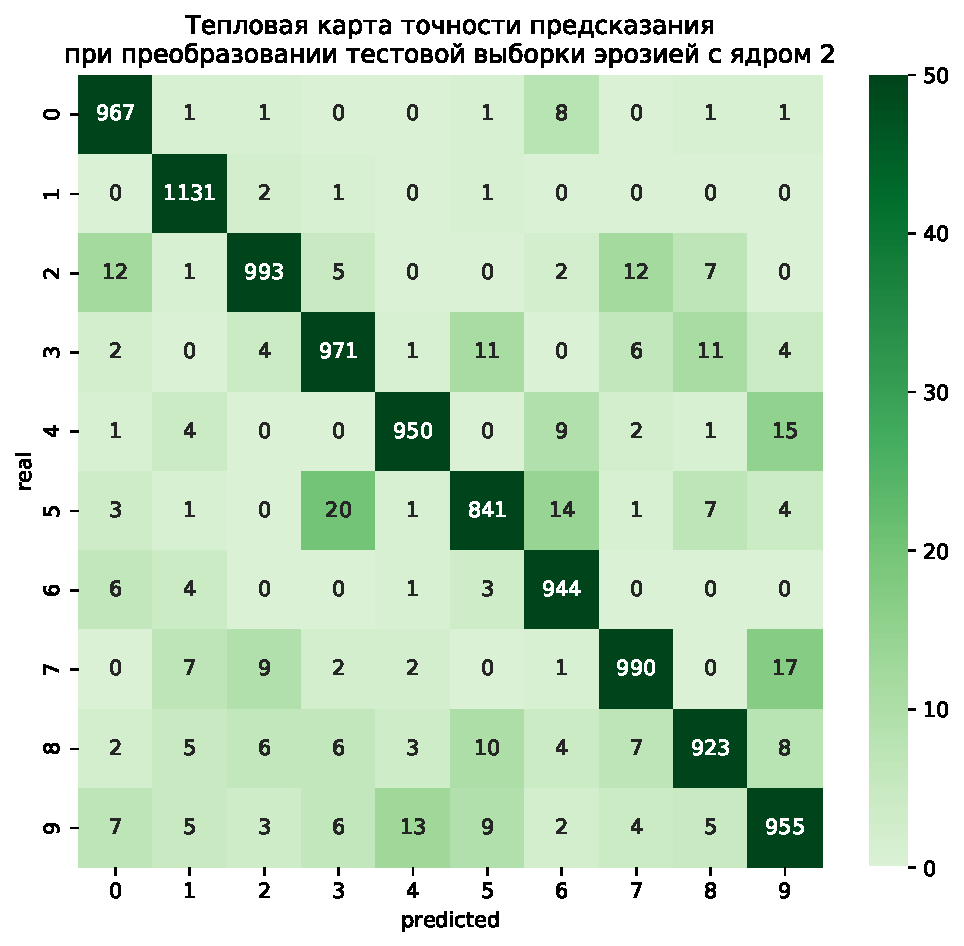
\includegraphics[scale=0.35]{TASK1 test morf1.pdf}
			% \caption{Caption}
		\end{minipage}
		\label{app6:morf1}
	}
	% \caption{Caption}
\end{figure}

\newpage
\begin{figure}[h]	
	\subfigure
	{
	    \begin{minipage}{8cm}
	        \centering
	        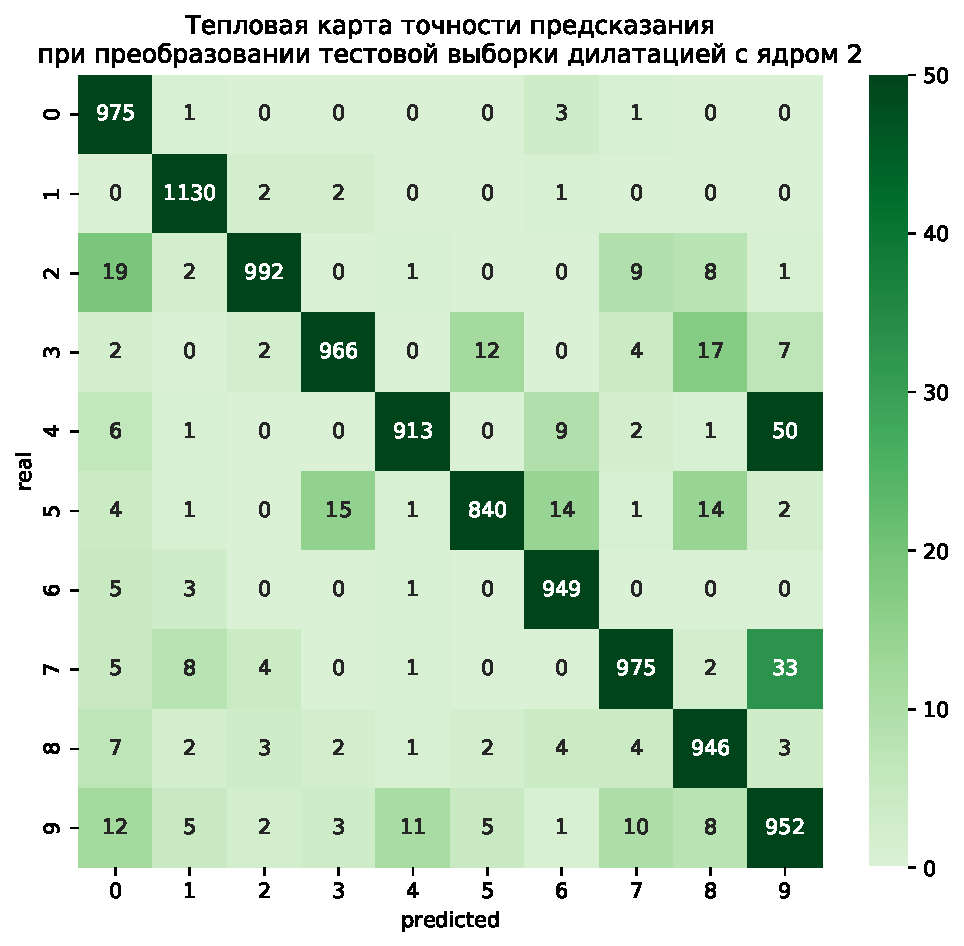
\includegraphics[scale=0.35]{TASK1 test morf2.pdf}
	        % \caption{Caption}
	    \end{minipage}
	    \label{app6:morf2}
	}
	\subfigure
	{
		\begin{minipage}{8cm}
			\centering
			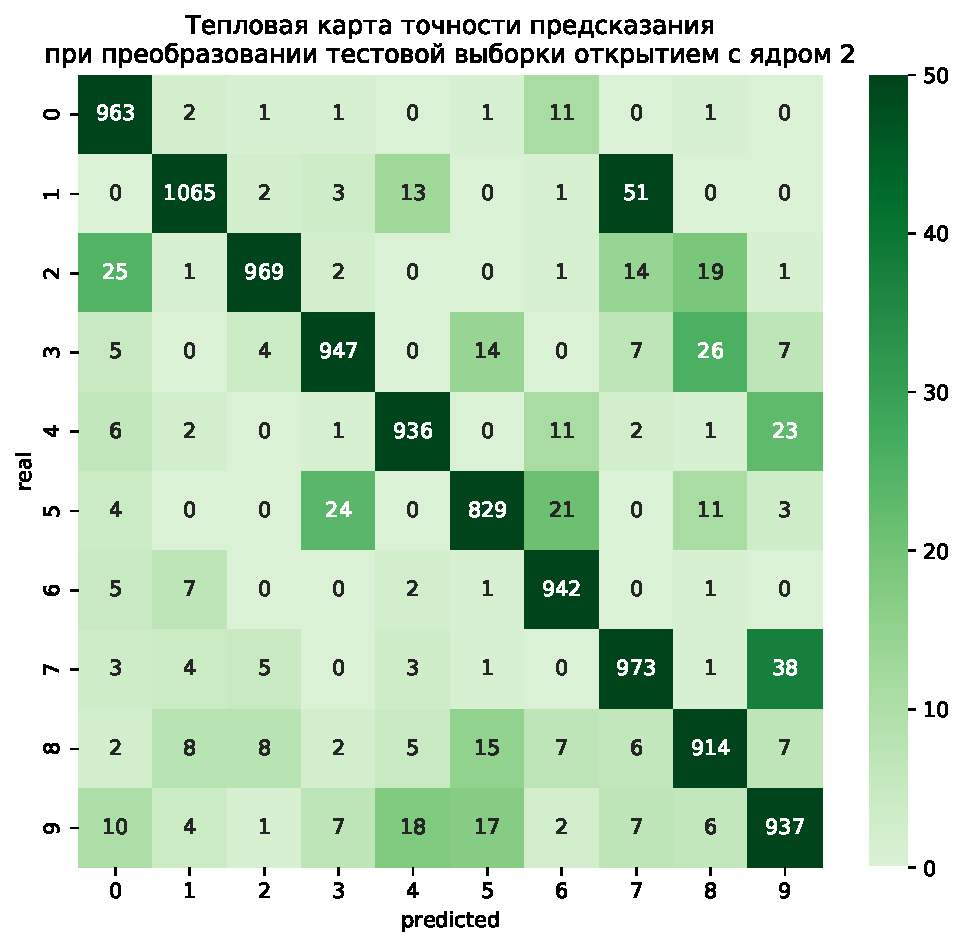
\includegraphics[scale=0.35]{TASK1 test morf3.pdf}
			% \caption{Caption}
		\end{minipage}
		\label{app6:morf3}
	}
	\subfigure
	{
	    \begin{minipage}{8cm}
	        \centering
	        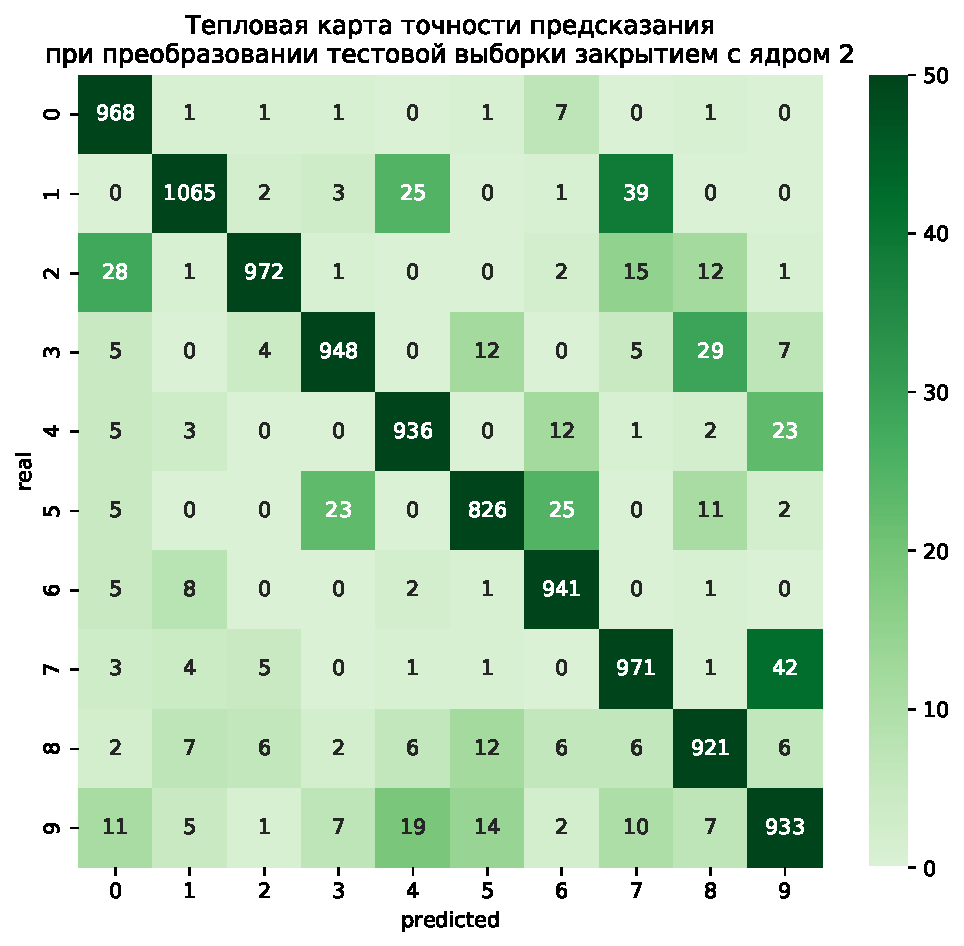
\includegraphics[scale=0.35]{TASK1 test morf4.pdf}
	        % \caption{Caption}
	    \end{minipage}
	    \label{app6:morf4}
	}
	% \caption{Caption}
\end{figure}




\newpage
\addcontentsline{toc}{section}{Список используемой литературы}
\begin{thebibliography}{}
    \bibitem{ss0} \href{https://ru.m.wikipedia.org/wiki/Метод_k-ближайших_соседей}{Википедия - метод K ближайших соседей}
    \bibitem{ss00} \href{http://www.machinelearning.ru/wiki/index.php?title=Метод_ближайшего_соседа}{Machinelearning - метод ближайшего соседа}
    \bibitem{ss1} \href{https://ml-handbook.ru/chapters/metric_based/intro}{Ml-handbook}
    \bibitem{ss2} \href{https://russianblogs.com/article/8928748181/}{Russianblogs}
    \bibitem{ss3} \href{https://www.kaggle.com/code/cdeotte/mnist-perfect-100-using-knn/notebook}{MNIST Perfect 100\% using kNN}
\end{thebibliography}

\end{document}